\chapter{Benchmarking QUBO solvers}\label{benchmark}

\section{Related benchmarking work}
One of the first benchmarking works for quantum annealing was conducted by Denchev et al. \yrcite{denchev2016computational}, who measured the performance of D-Wave quantum annealing on the older D-Wave 2X machine using specially crafted problems that have tall and narrow energy barriers separating local minima. Quantum annealing is expected to be $1.8 \times 10^8$ times faster compared to simulated annealing, which tends to fail with problems with such an energy landscape.


\outcite{b34} evaluated the performance of QAOA on the IBMQ backend and the D-Wave quantum annealer using instances of MaxCut and 2-satisfiability problems with up to 18 variables. The performance of the QAOA algorithm is inconsistent and underperforms quantum annealing in their problem set. More recently, \outcite{b35} also compared the performance of QAOA on the IBMQ backend and D-Wave quantum annealing on randomly generated Ising problems with cubic interaction terms and also found that quantum annealing had superior performance over QAOA for all problem sizes. 

\outcite{gomes2019classical} showed that the NNQS solver with an RBM architecture produces good solutions for the max-cut problem with graph sizes of up to 256. \outcite{khandoker2023supplementing} uses recurrent neural networks as the NNQS architecture for the max-cut and traveling salesman problem and found that it outperforms SA. However, there is no direct study that compares performance across quantum annealing, QAOA, and NNQS.

\section{Results and Discussion}
\subsection{NAE3SAT}

\begin{figure}[!htbp]
    \subfloat[Normalized energy]{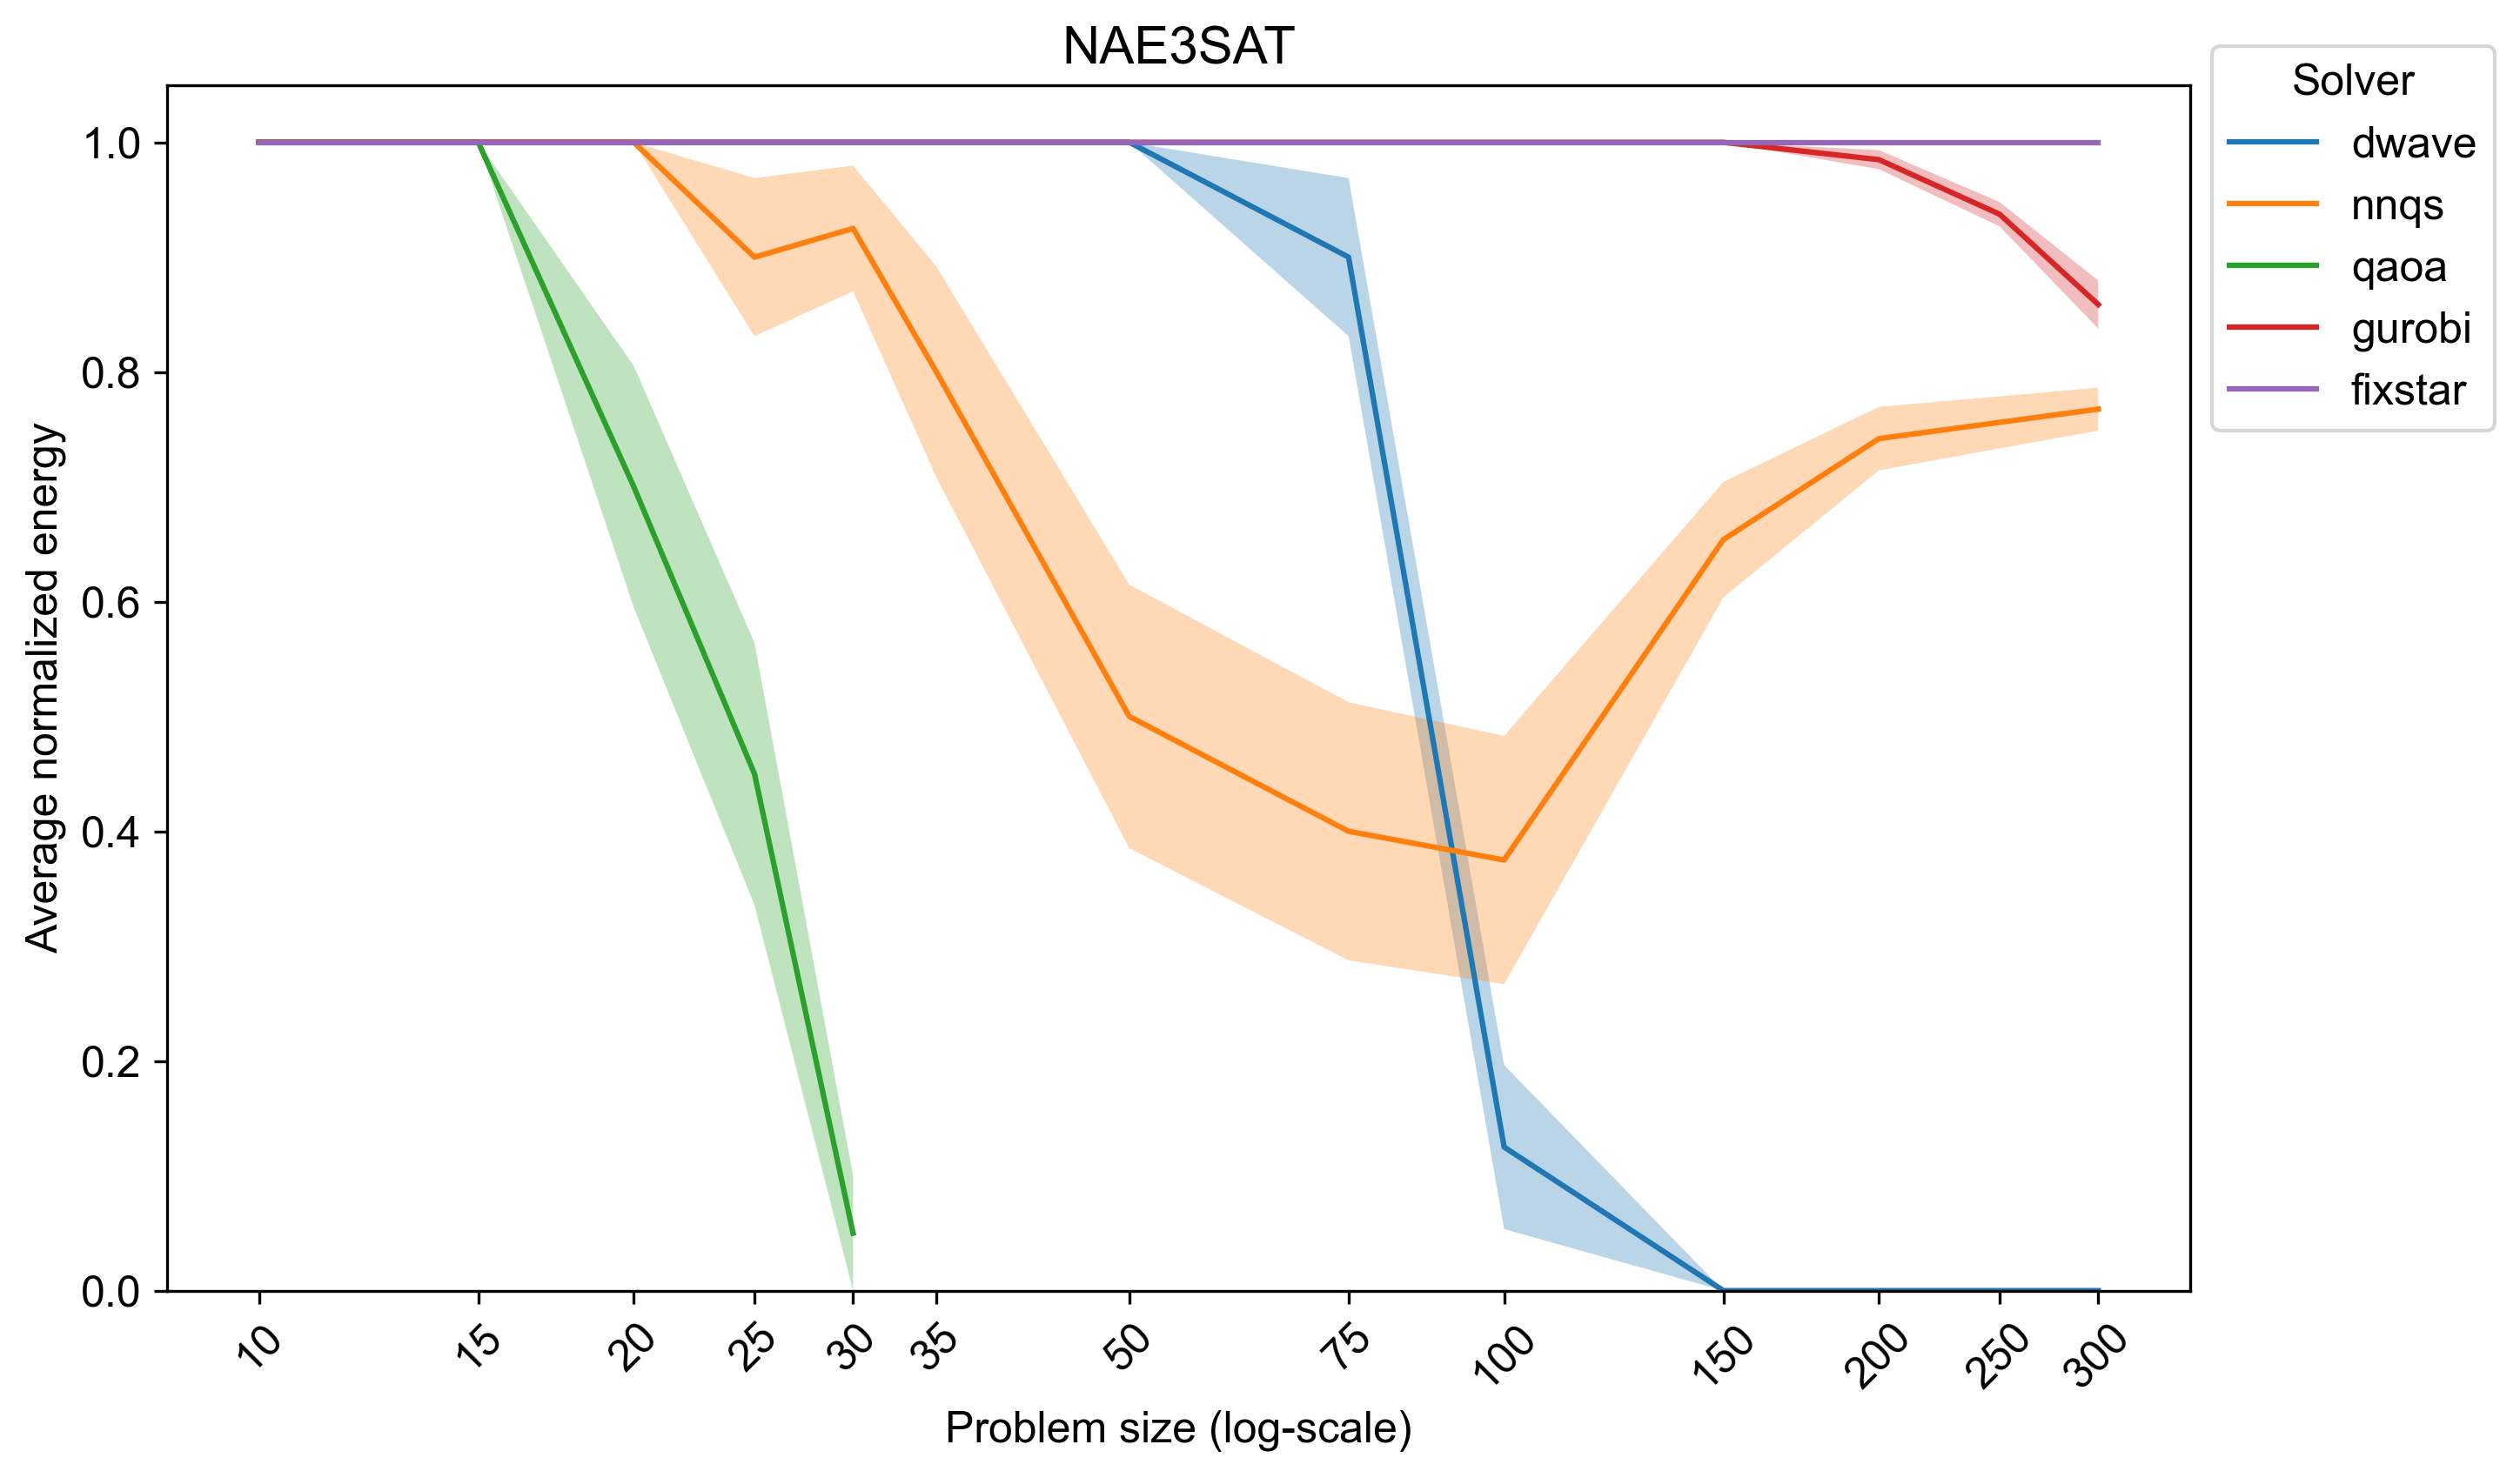
\includegraphics[width=0.9\textwidth]{images/nae3sat_all_size.png}}
    \\
    \subfloat[Success probability]{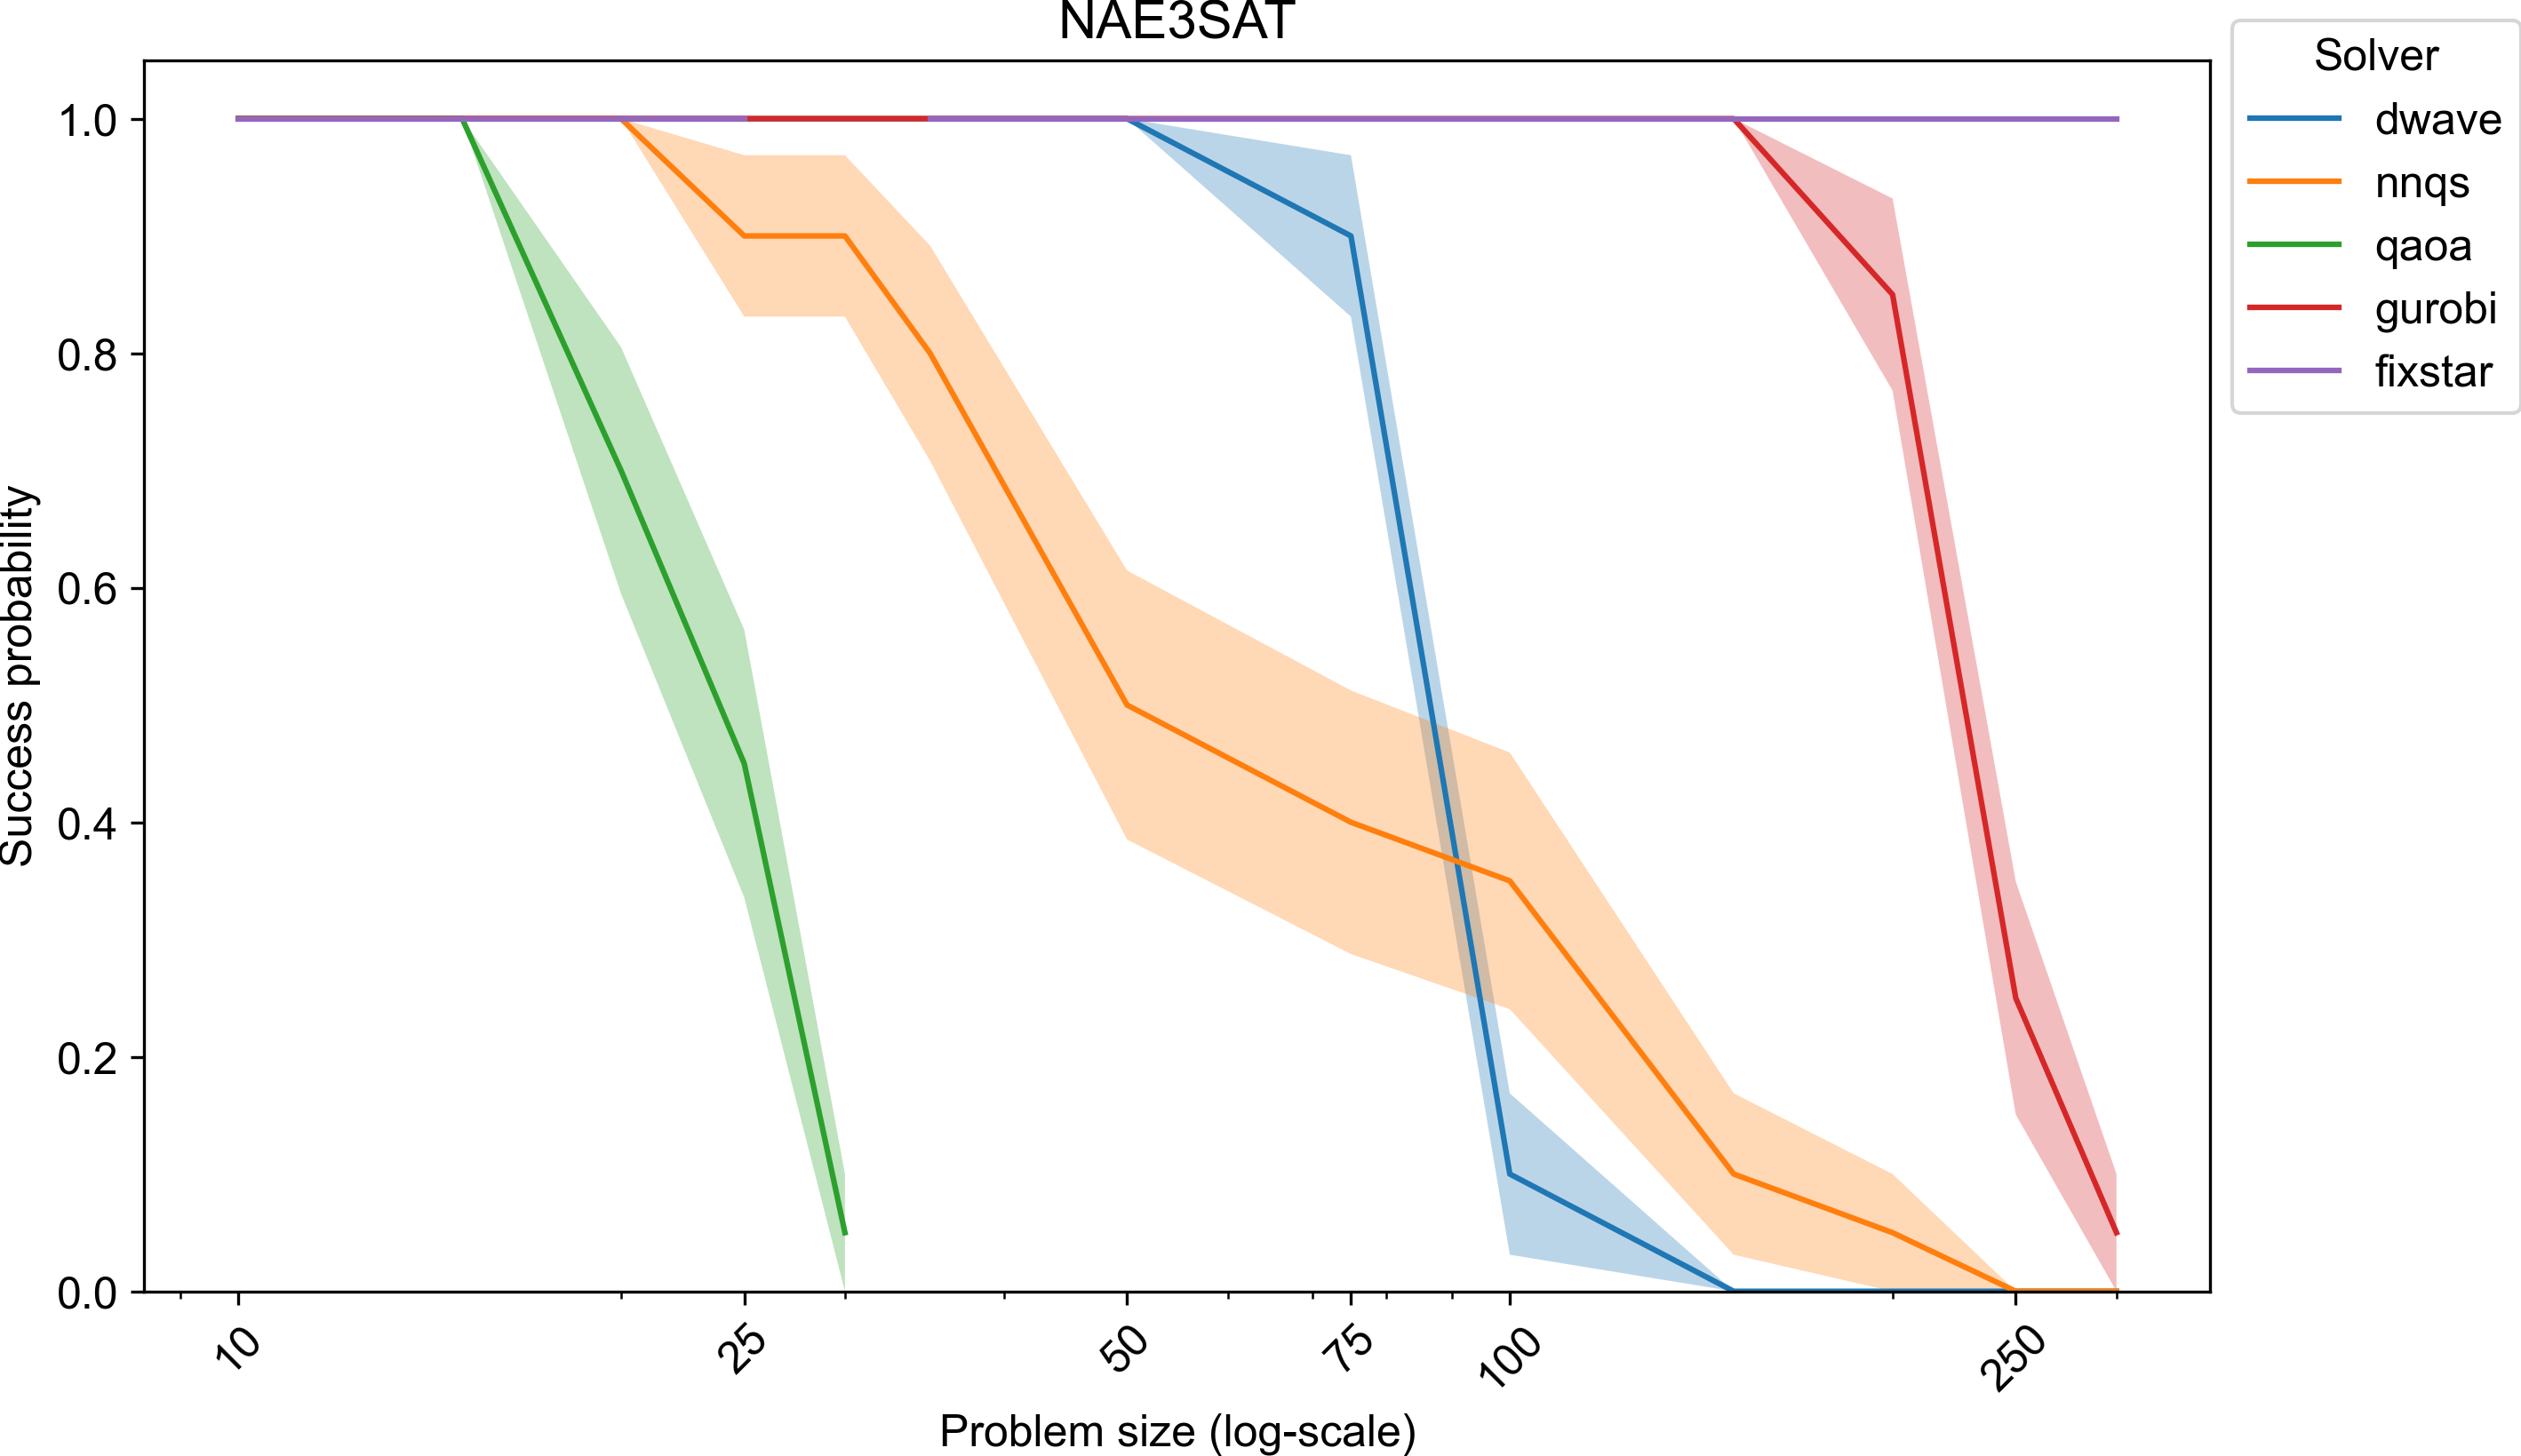
\includegraphics[width=0.9\textwidth]{images/nae3sat_all_success_size.png}}
    \caption{Performance of different solvers for NAE3SAT by problem size}
    \label{all-nae3sat-size}
\end{figure}

\begin{figure}[!htbp]
    \subfloat[Normalized energy]{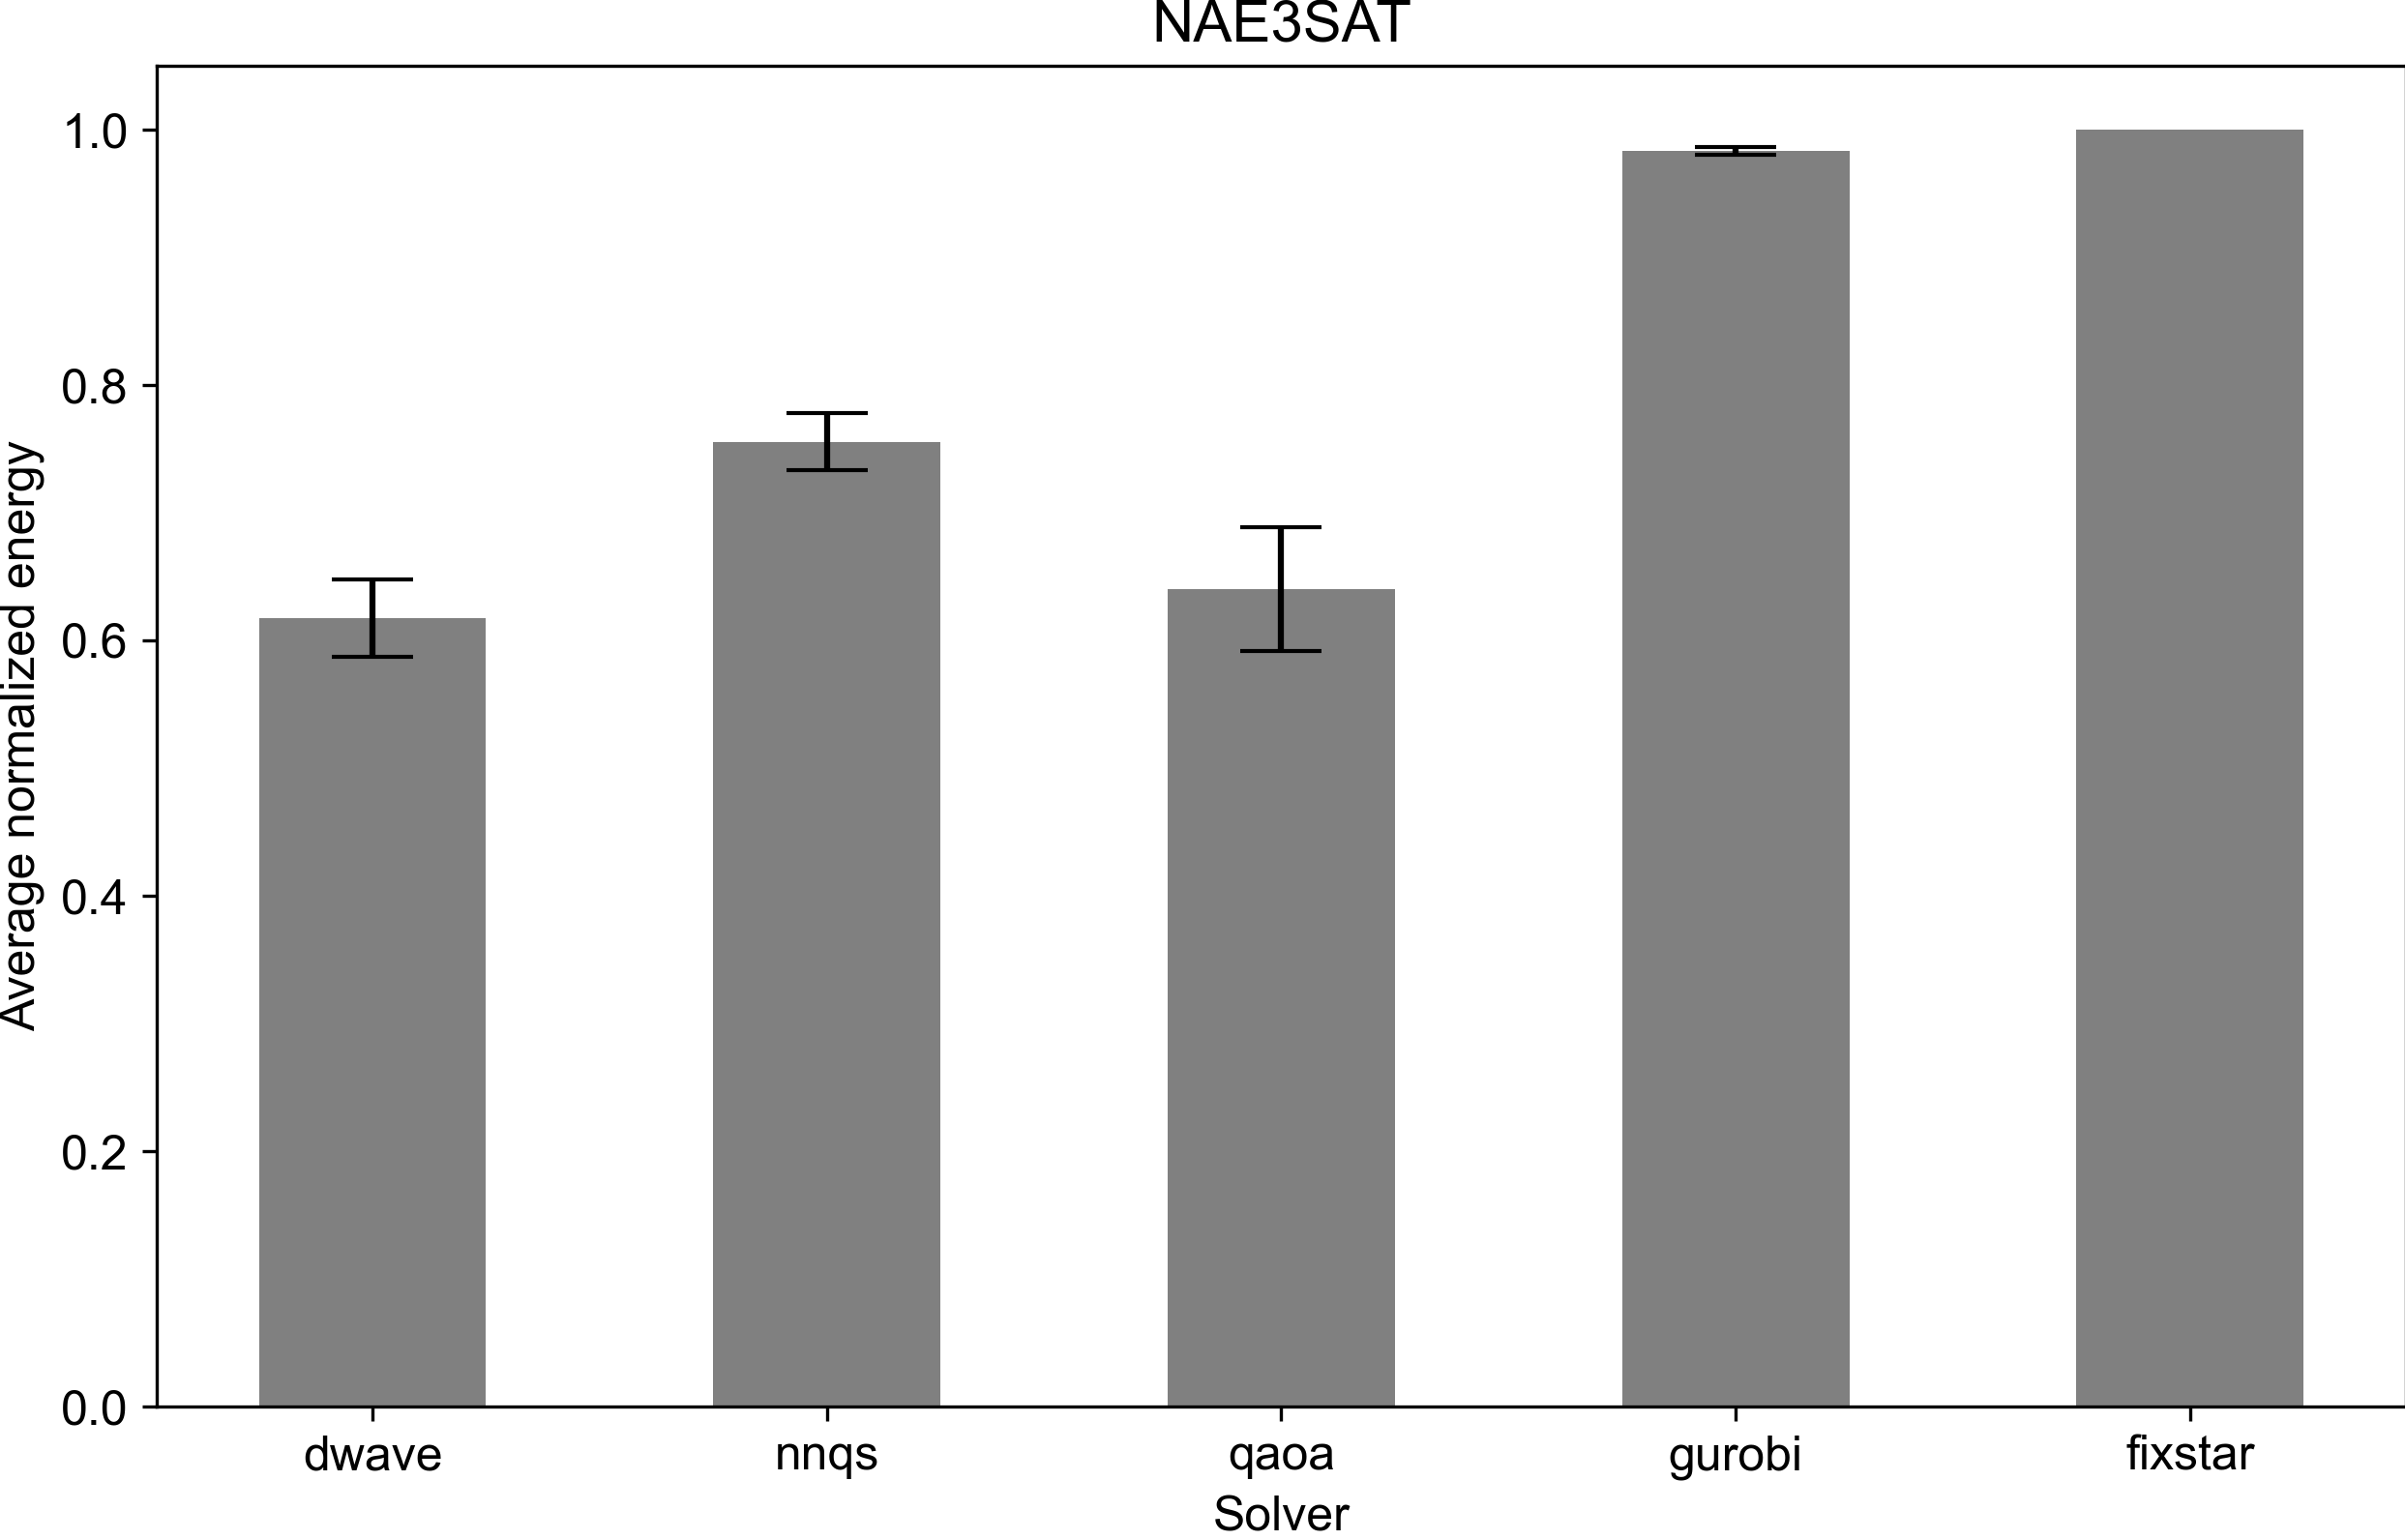
\includegraphics[width=0.49\textwidth]{images/nae3sat_all_avg.png}}\hfill
    \subfloat[Success probability]{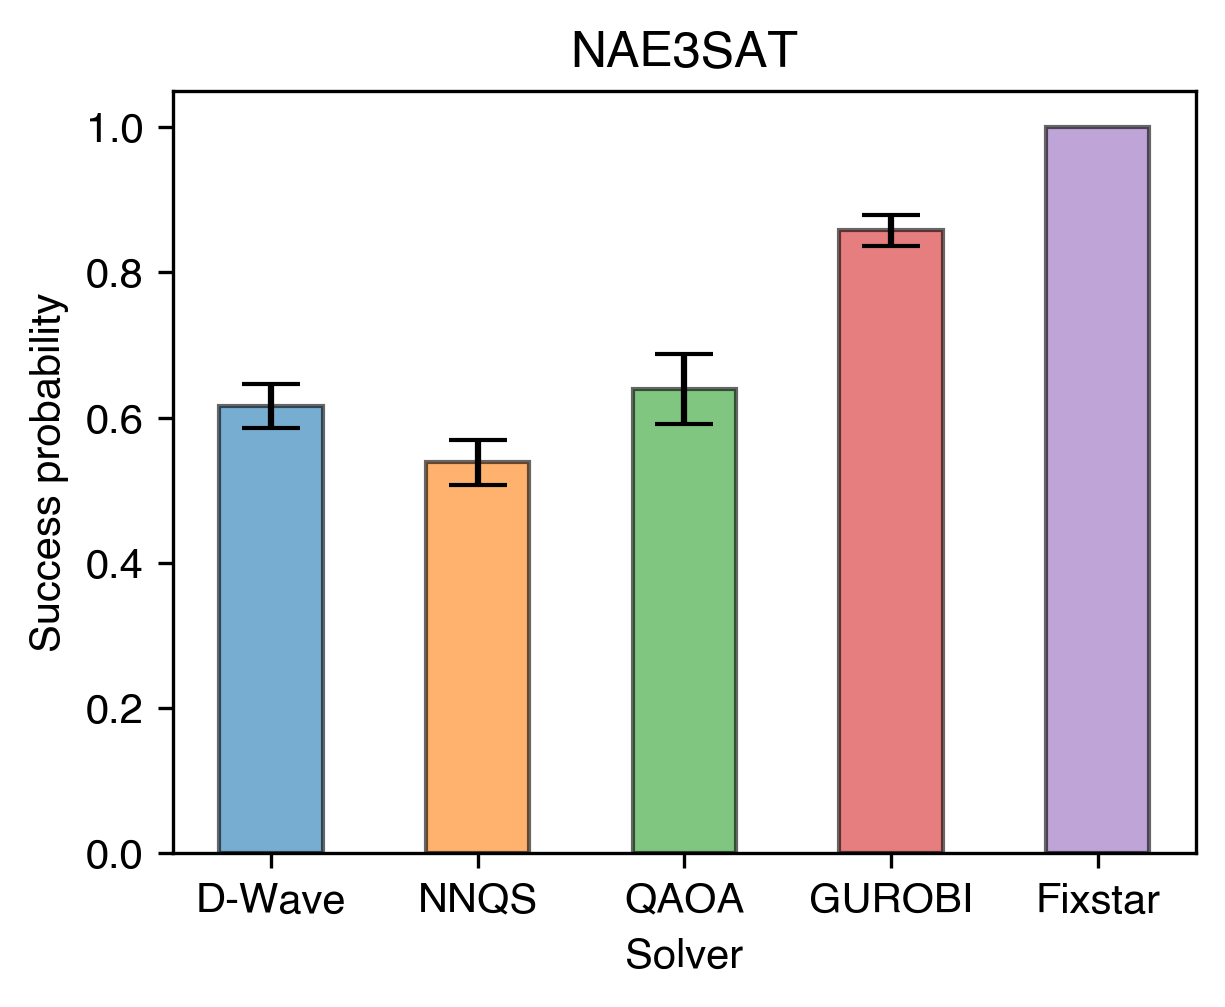
\includegraphics[width=0.49\textwidth]{images/nae3sat_all_success_avg.png}}
    \caption{Average performance of different solvers for NAE3SAT}
    \label{all-nae3sat-average}
\end{figure}

For the NAE3SAT dataset, the continuous training algorithm with the RBM performed the best in terms of normalized energy and success probability, shown in \autoref{all-nae3sat-size}, except with a problem size of $50$. This is likely due to variance in the randomly generated data set. The performance averaged across all sizes, shown in \autoref{all-nae3sat-average}, also highlights that the RBM with a continuous training algorithm performs the best.

\subsection{Max-cut}

\begin{figure}[!htbp]
    \subfloat[Normalized energy]{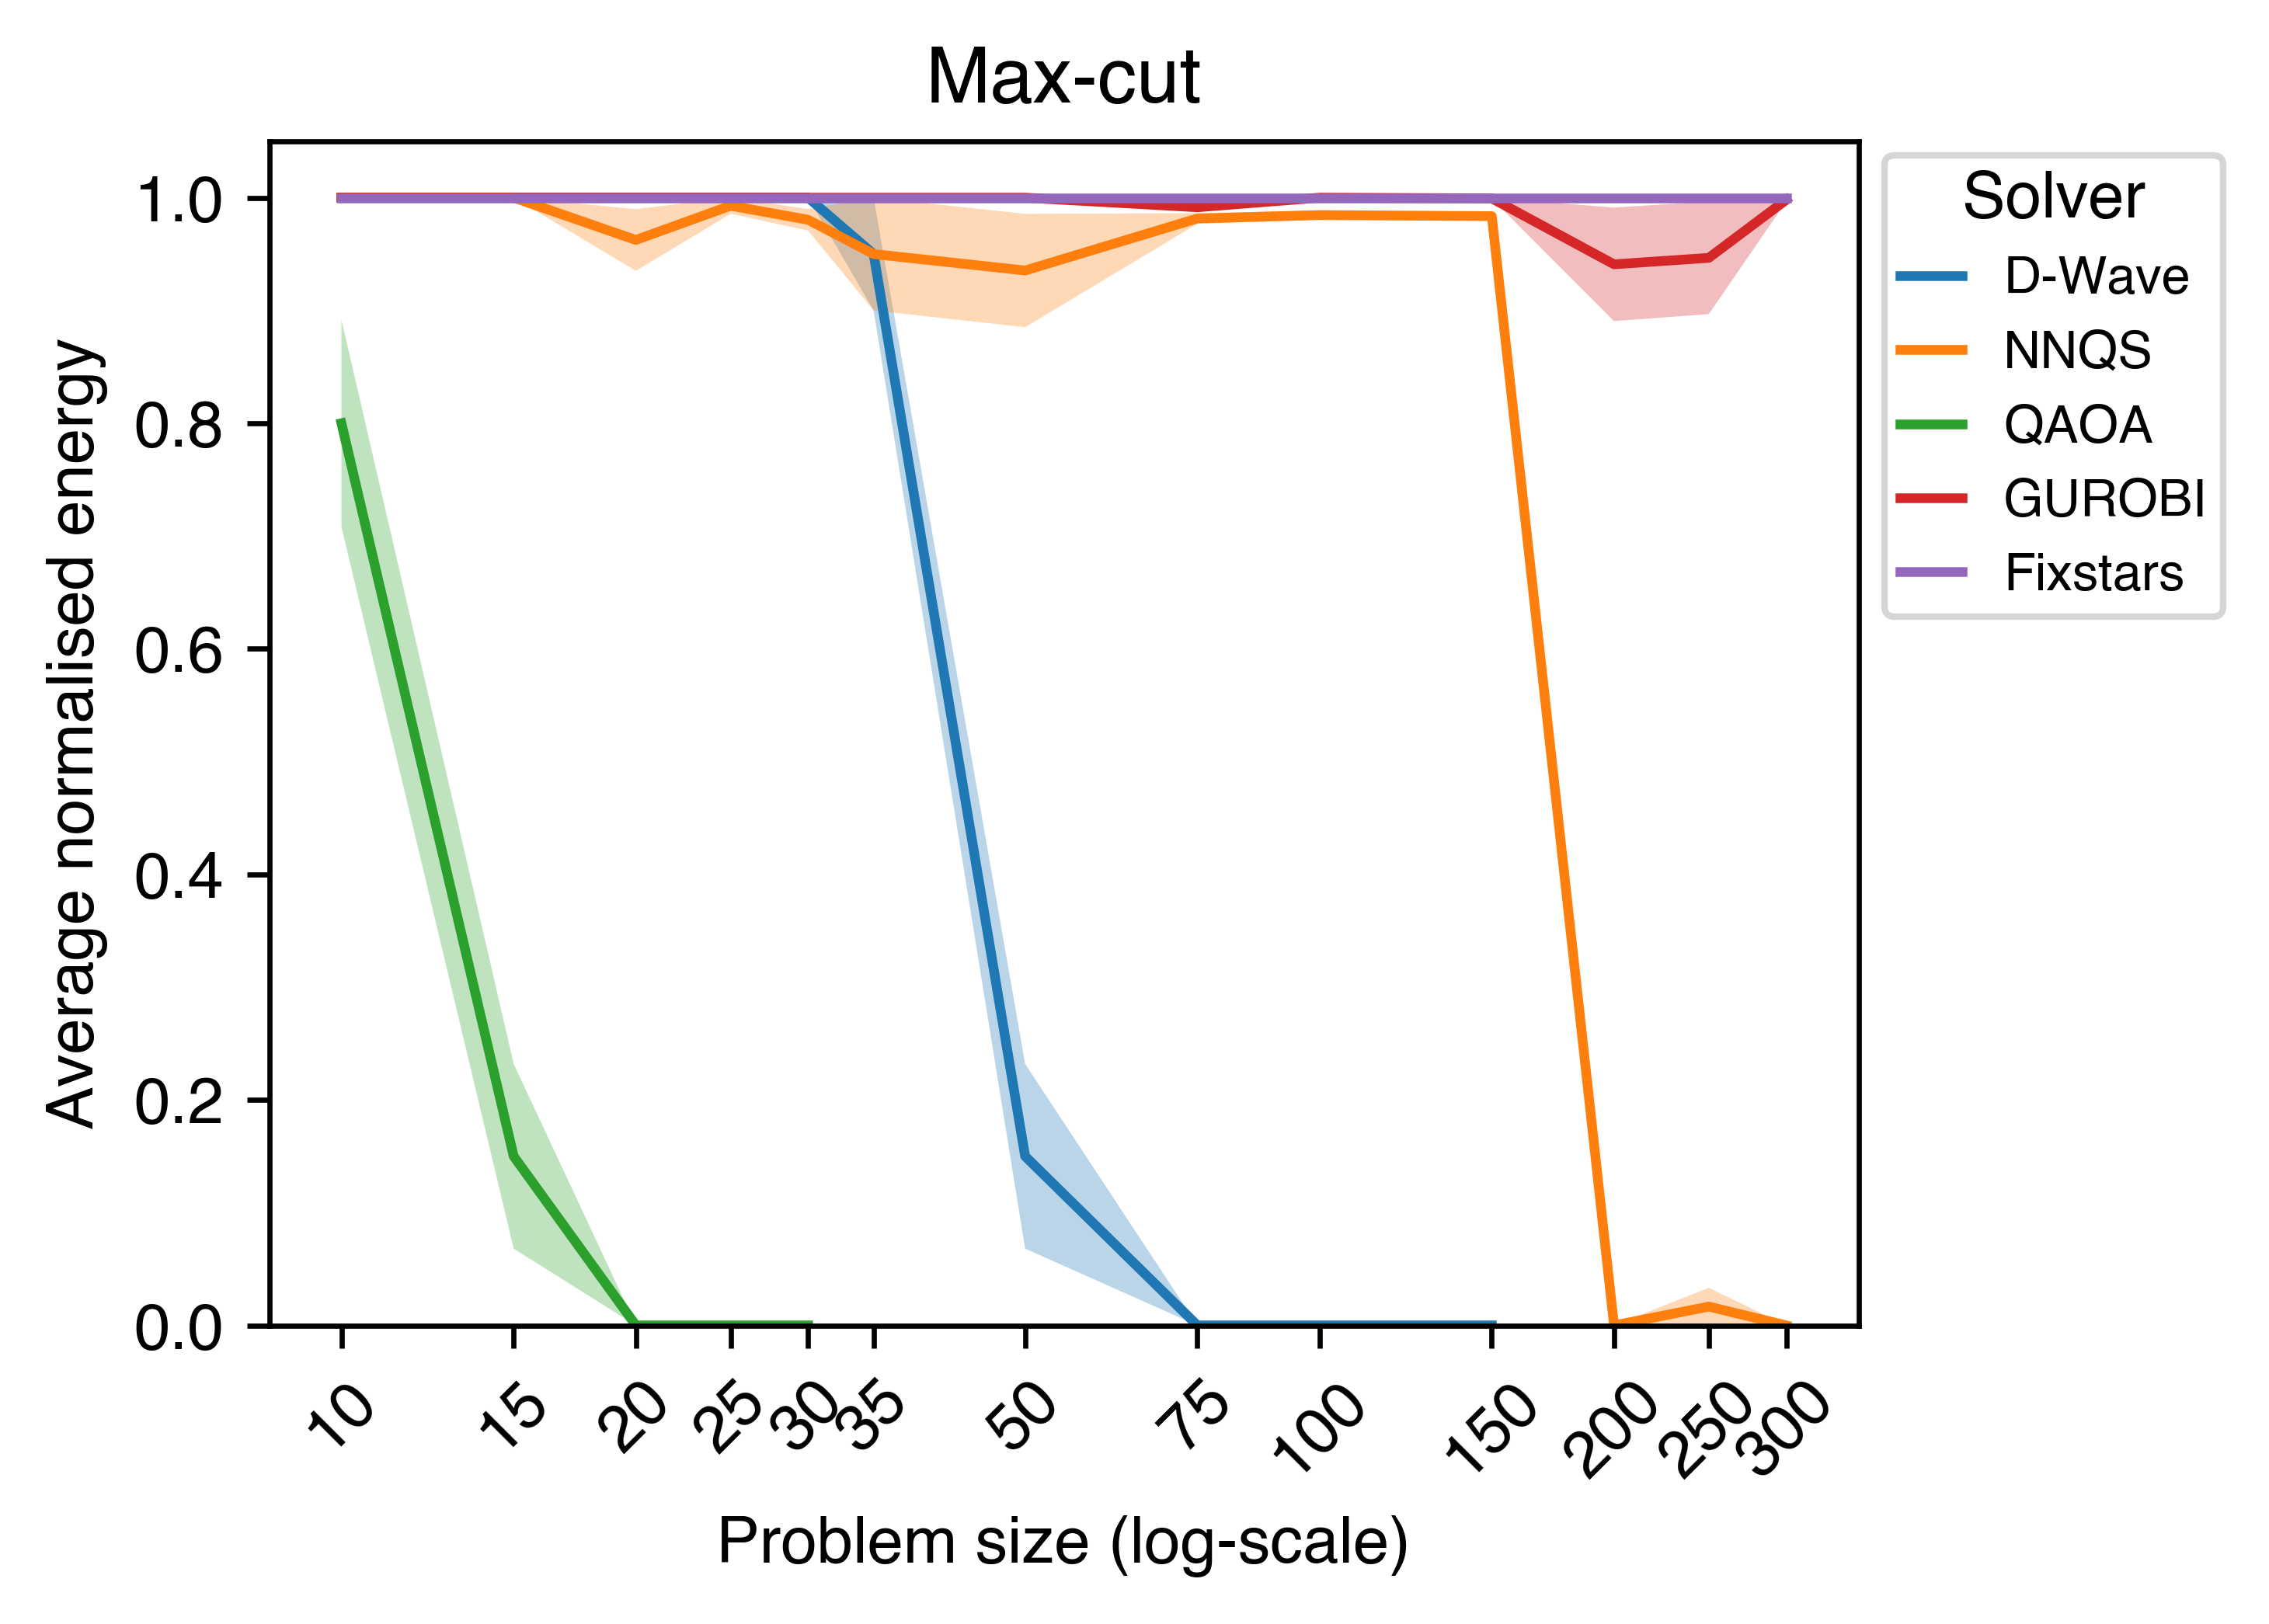
\includegraphics[width=0.9\textwidth]{images/maxcut_all_size.png}}
    \\
    \subfloat[Success probability]{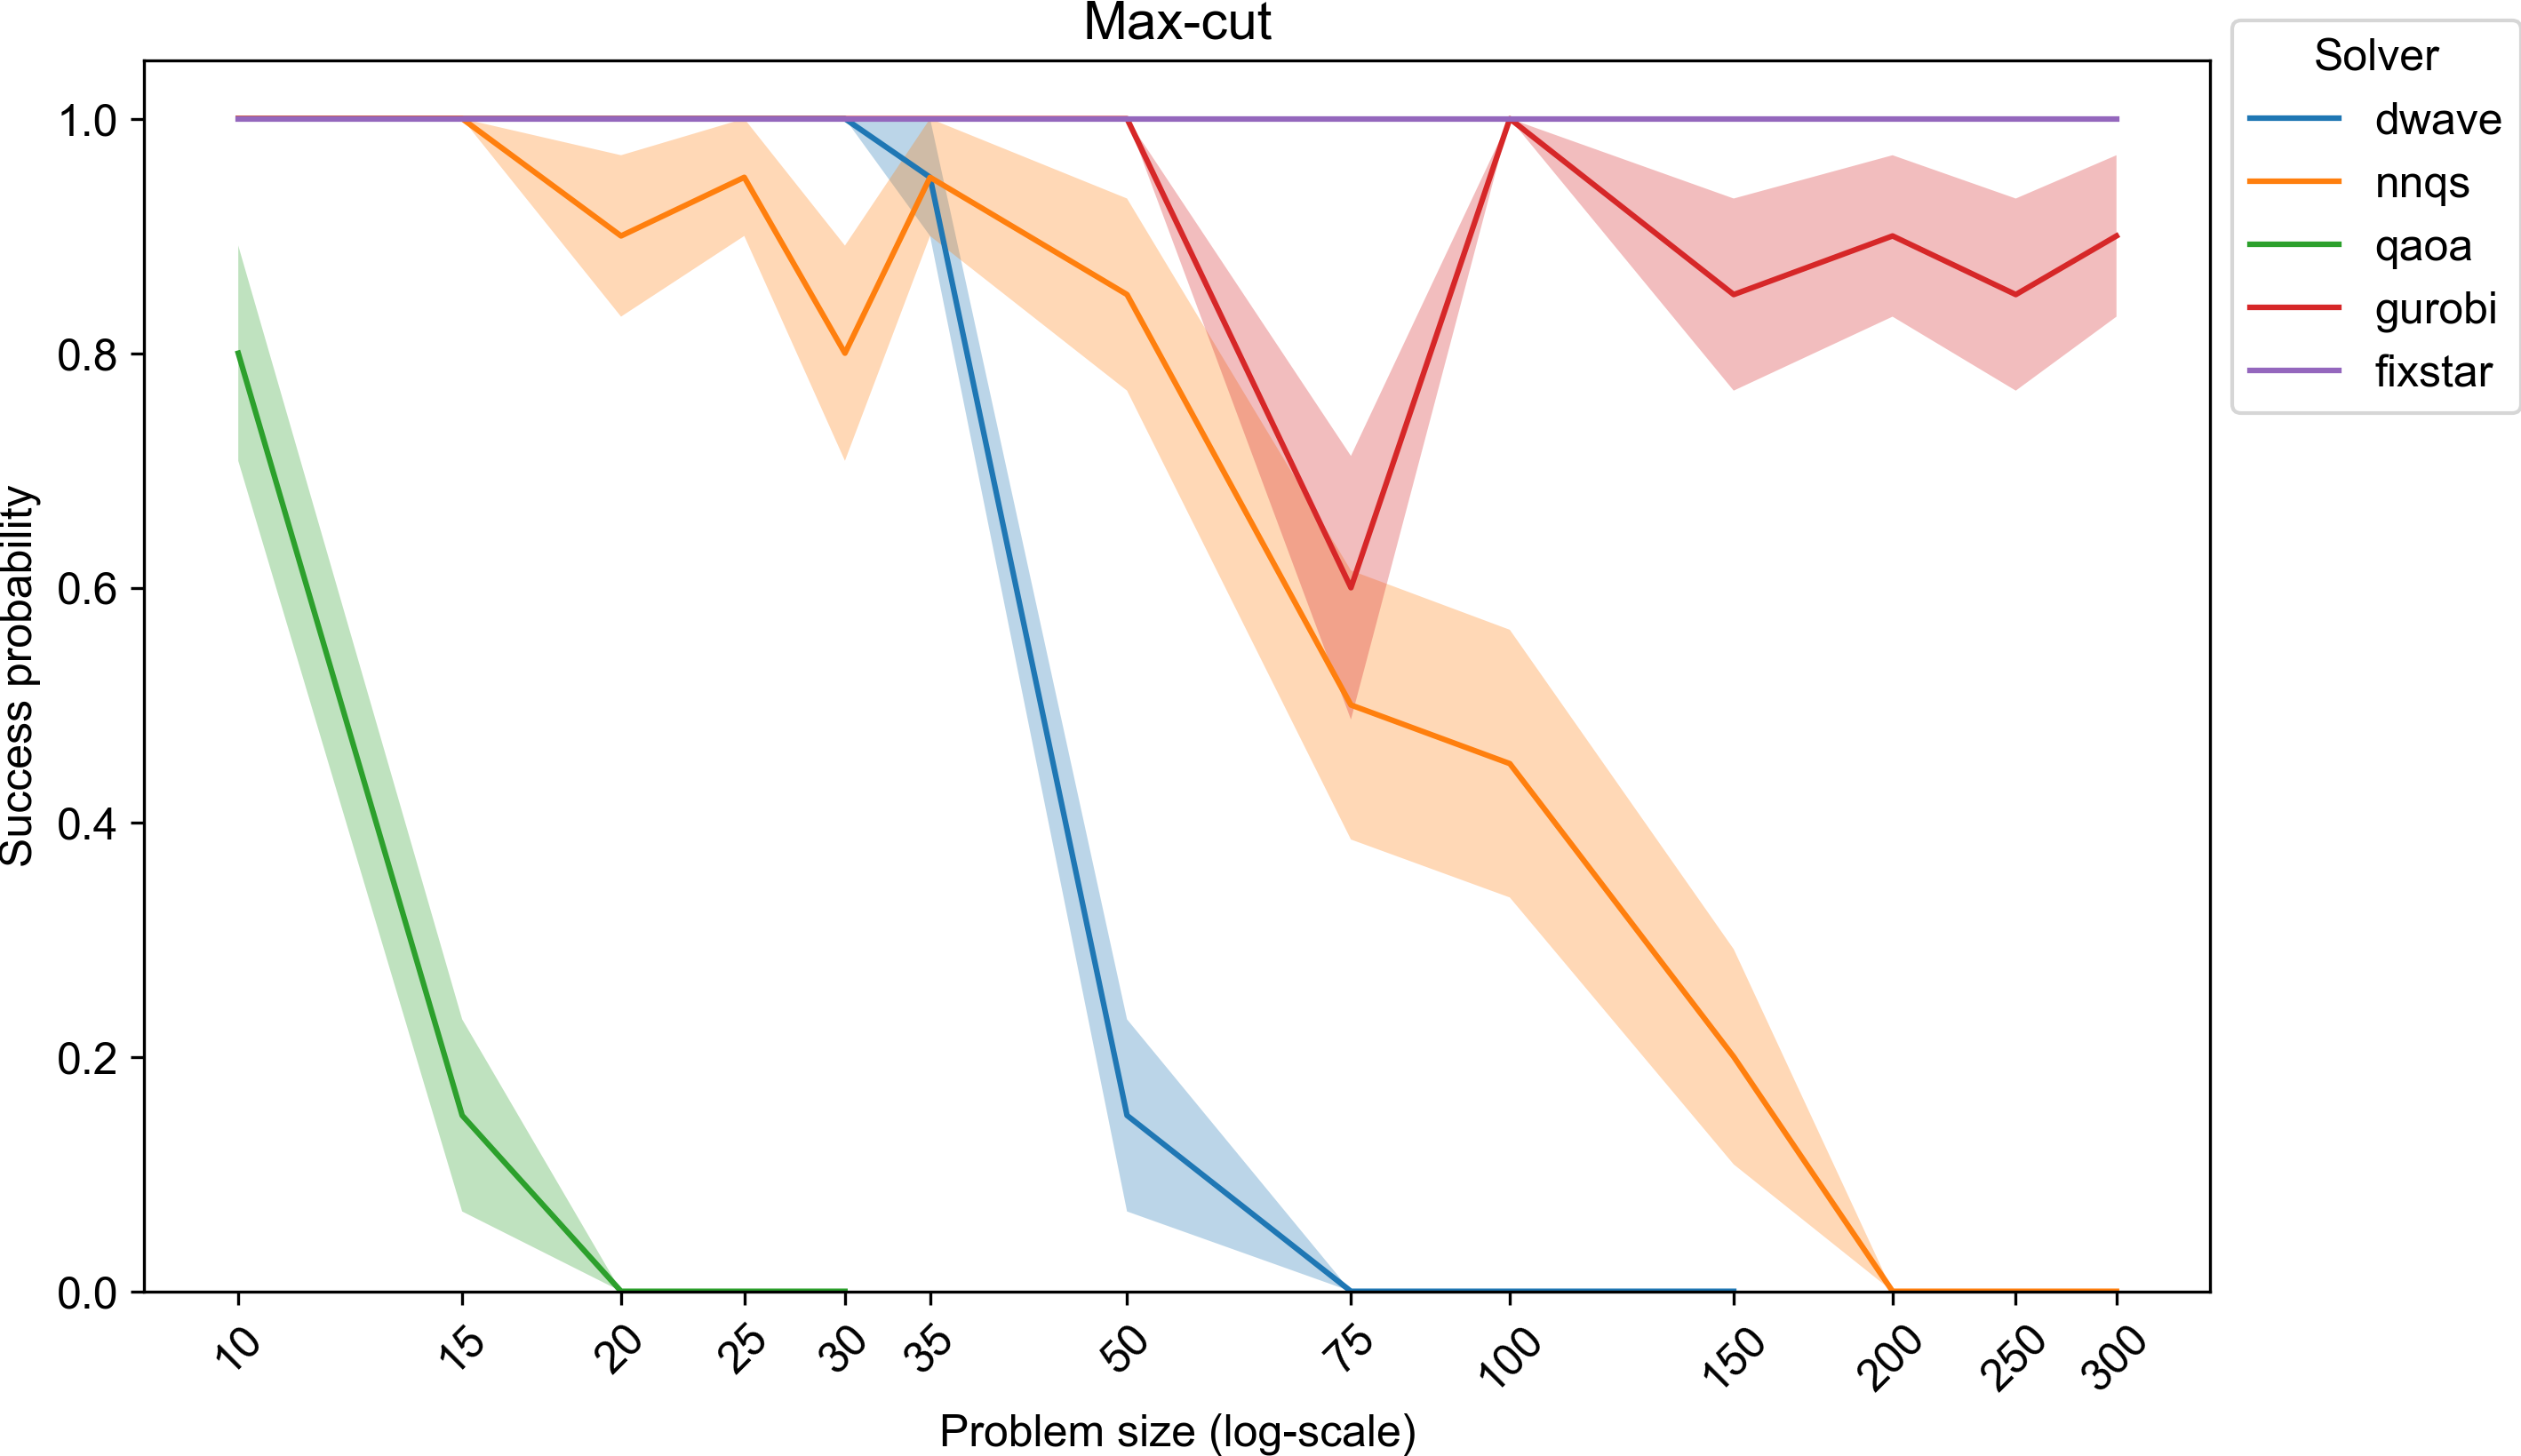
\includegraphics[width=0.9\textwidth]{images/maxcut_all_success_size.png}}
    \caption{Performance of different solvers for max-cut by problem size}
    \label{all-maxcut-size}
\end{figure}

\begin{figure}[!htbp]
    \subfloat[Normalized energy]{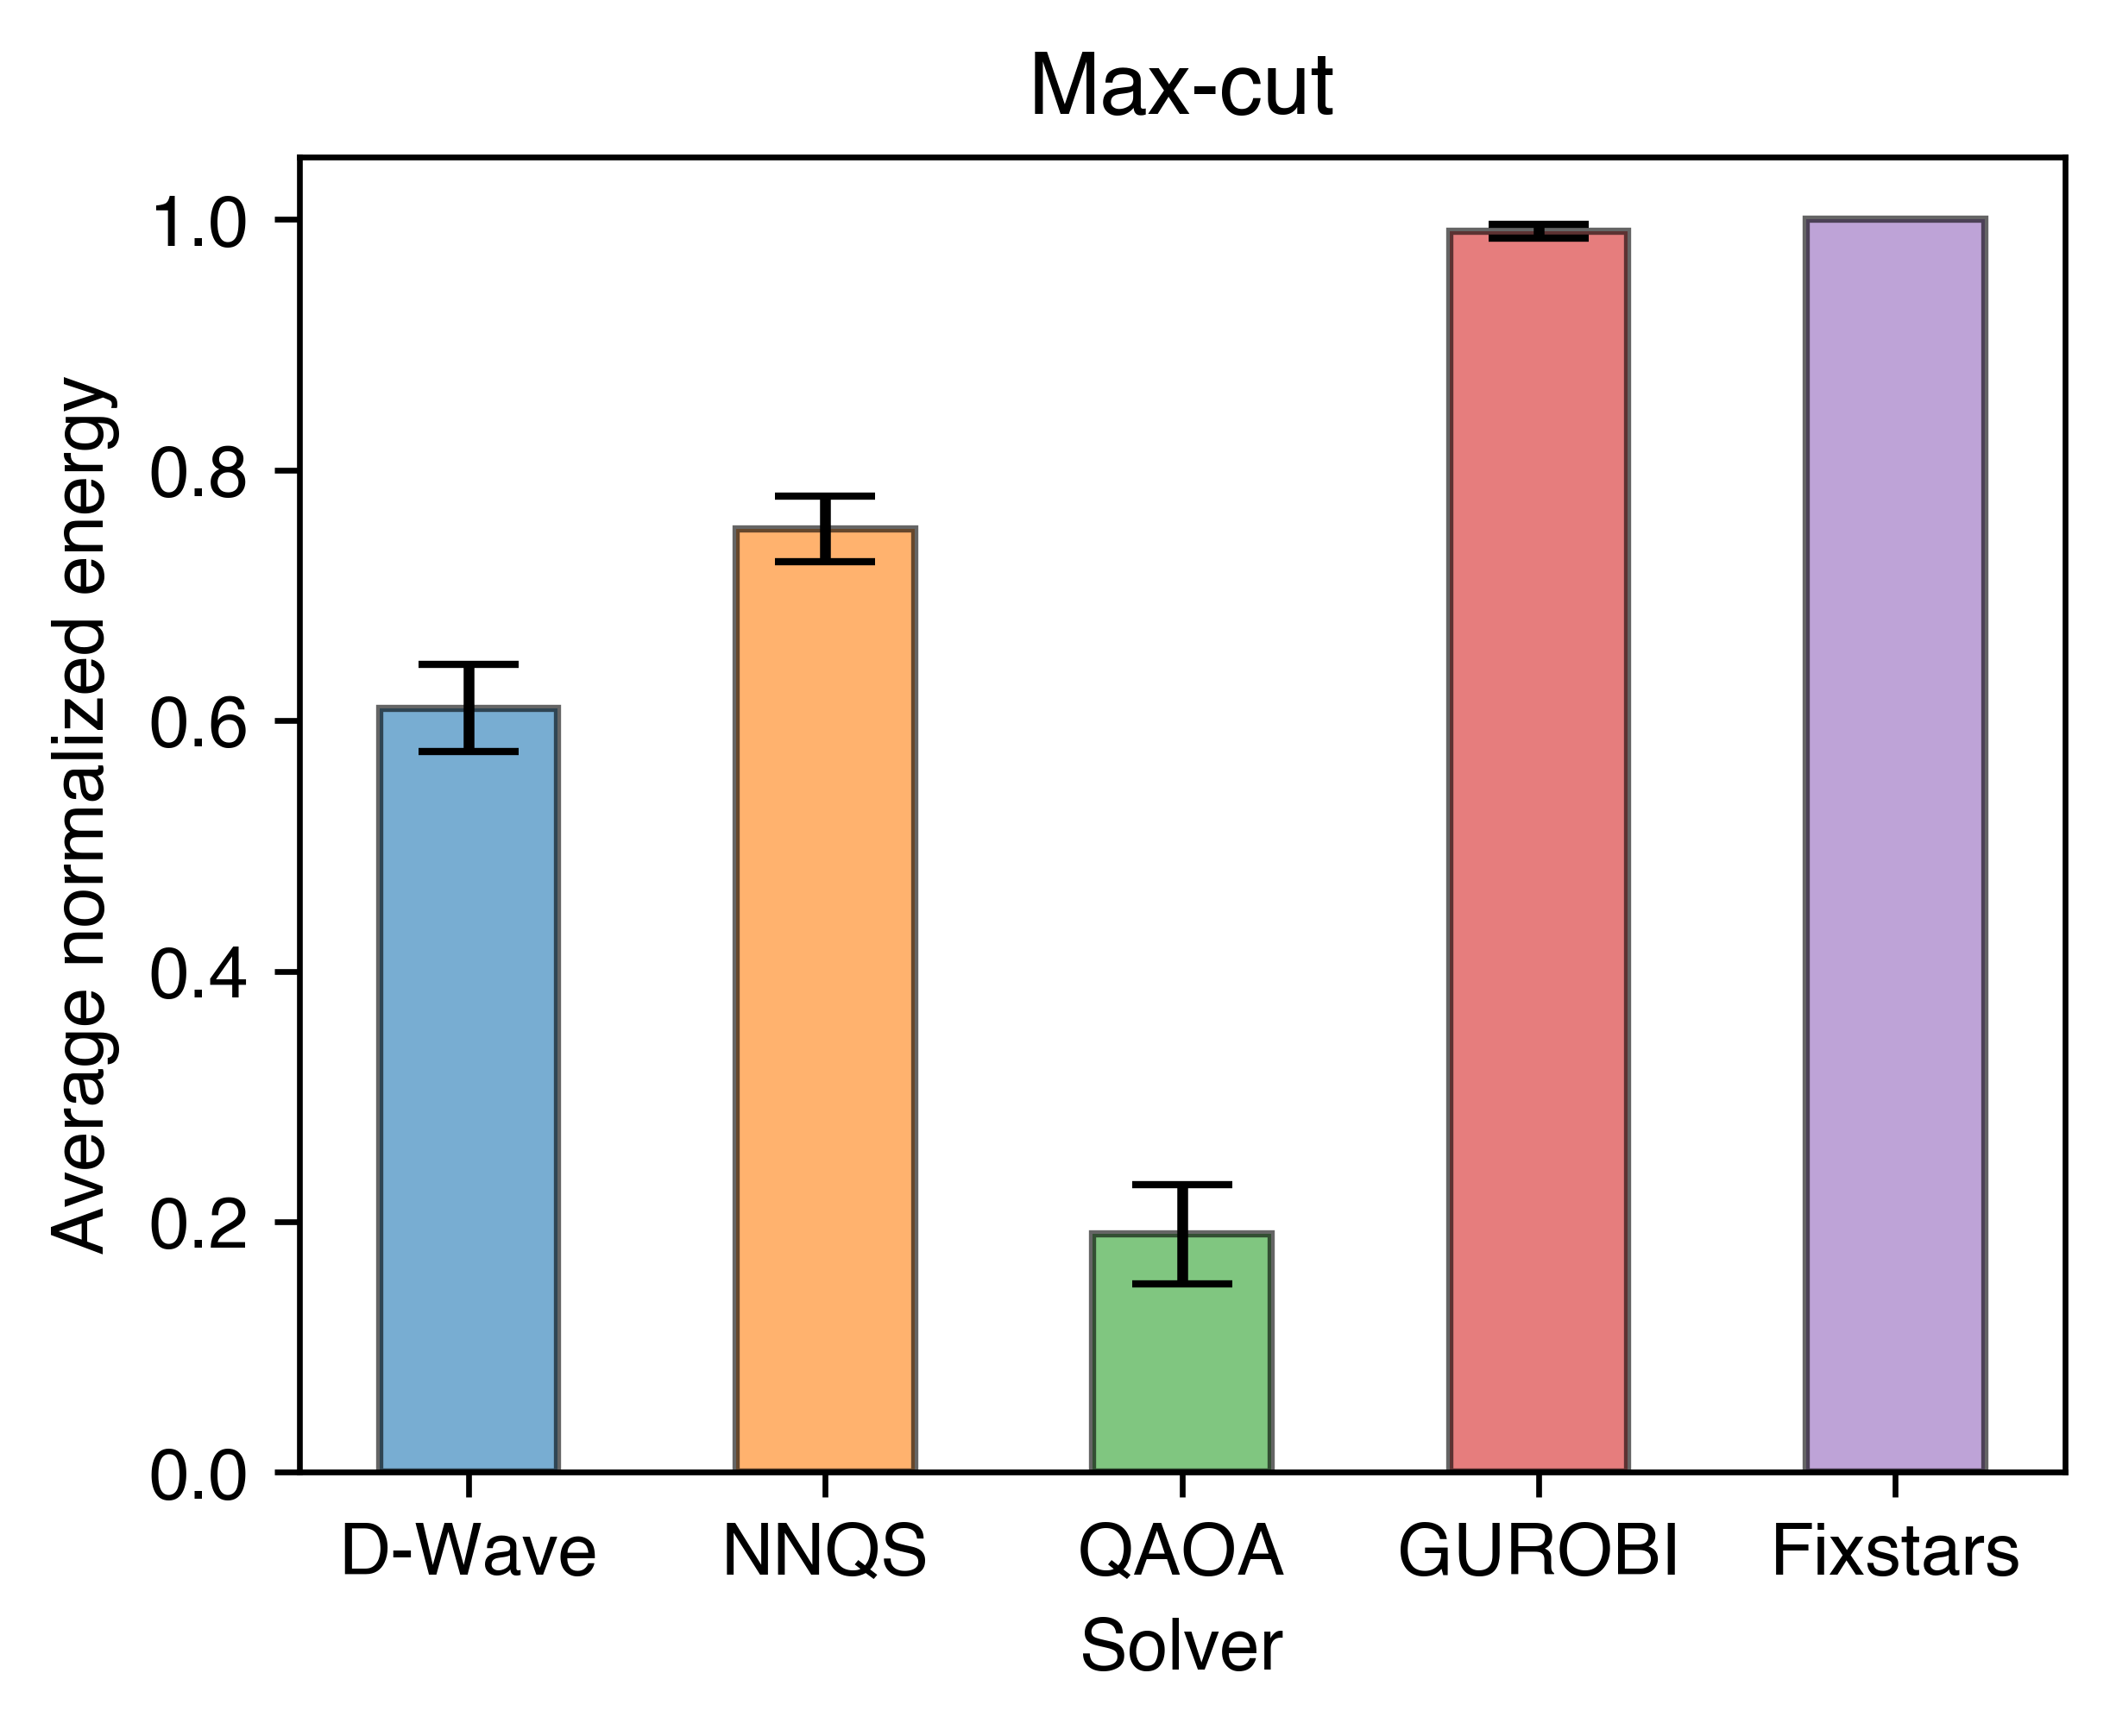
\includegraphics[width=0.49\textwidth]{images/maxcut_all_avg.png}}\hfill
    \subfloat[Success probability]{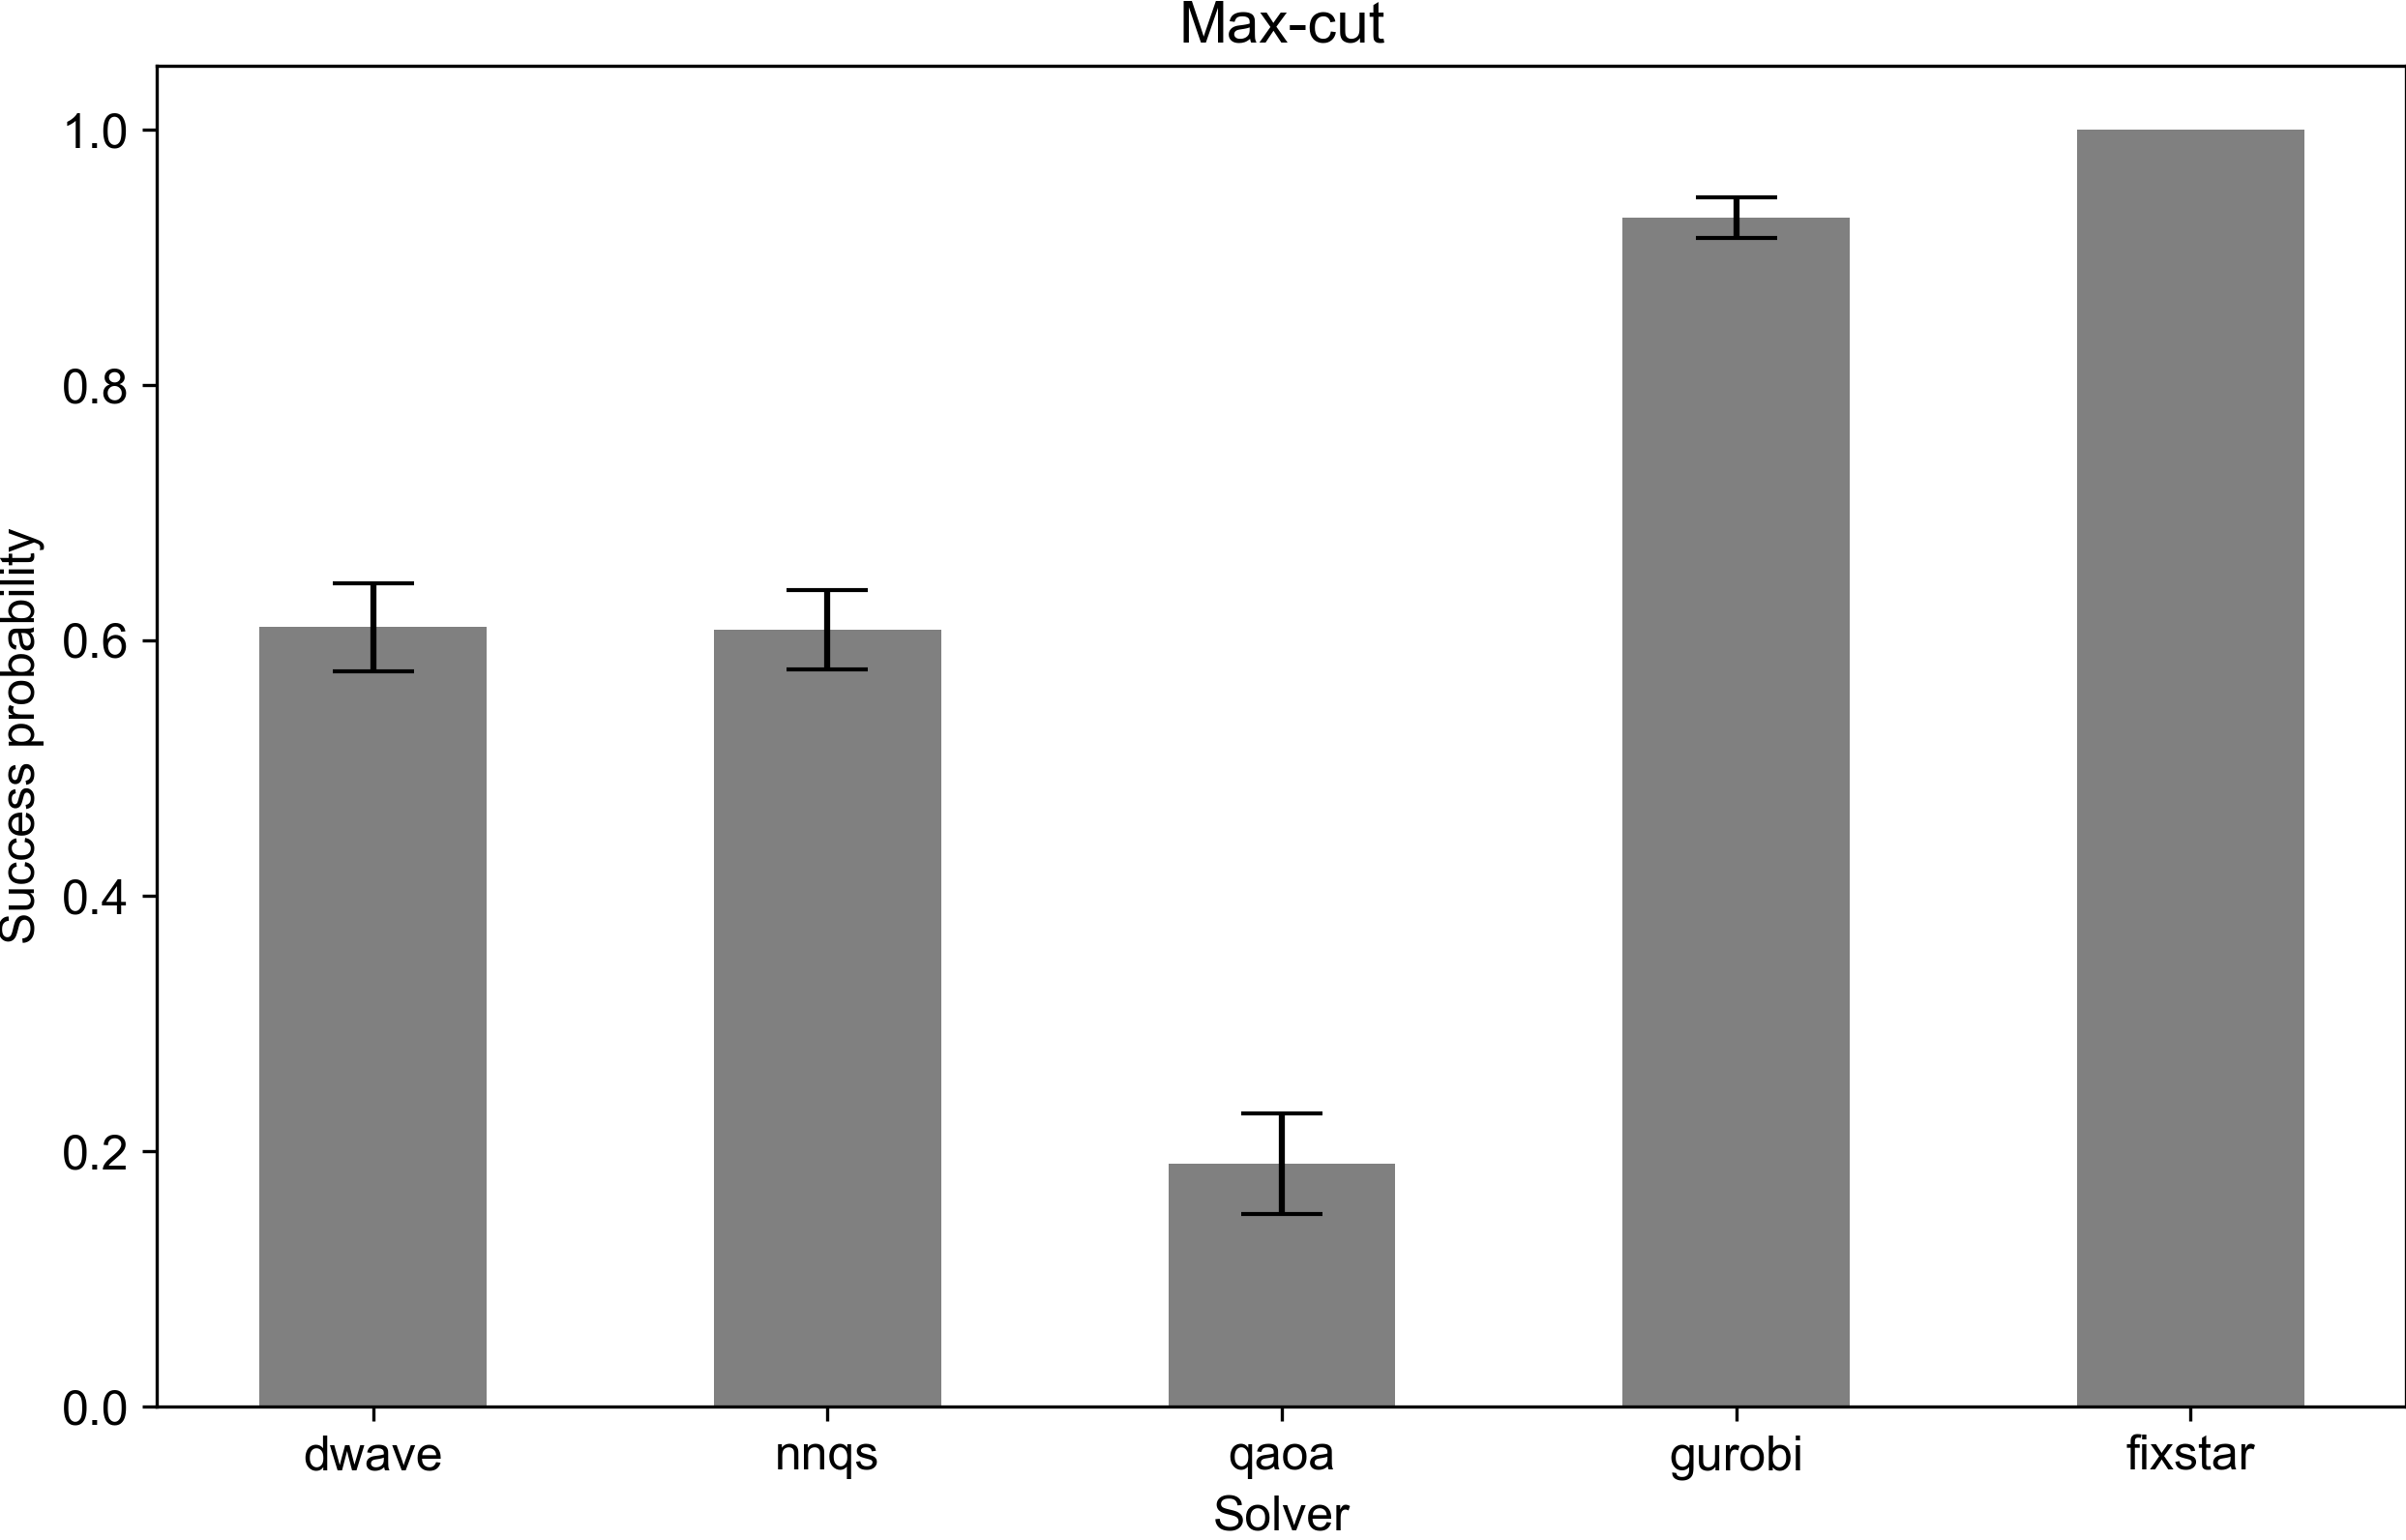
\includegraphics[width=0.49\textwidth]{images/maxcut_all_success_avg.png}}
    \caption{Average performance of different solvers for max-cut}
    \label{all-maxcut-average}
\end{figure}

For the max-cut dataset, the continuous training algorithm with the RBM generally performed the best in terms of normalized energy and success probability, shown in \autoref{all-maxcut-size}, except with a problem size of $25$. This is likely due to variance in the randomly generated data set. The performance averaged across all sizes, shown in \autoref{all-maxcut-average}, also highlights that the RBM with a continuous training algorithm performs the best. However, the gap in success probability between the models is relatively small and this likely implies that the max-cut problem is easier in general compared to the NAE3SAT problem.


\subsection{SK model}

\begin{figure}[!htbp]
    \centering
    \subfloat[Normalized energy]{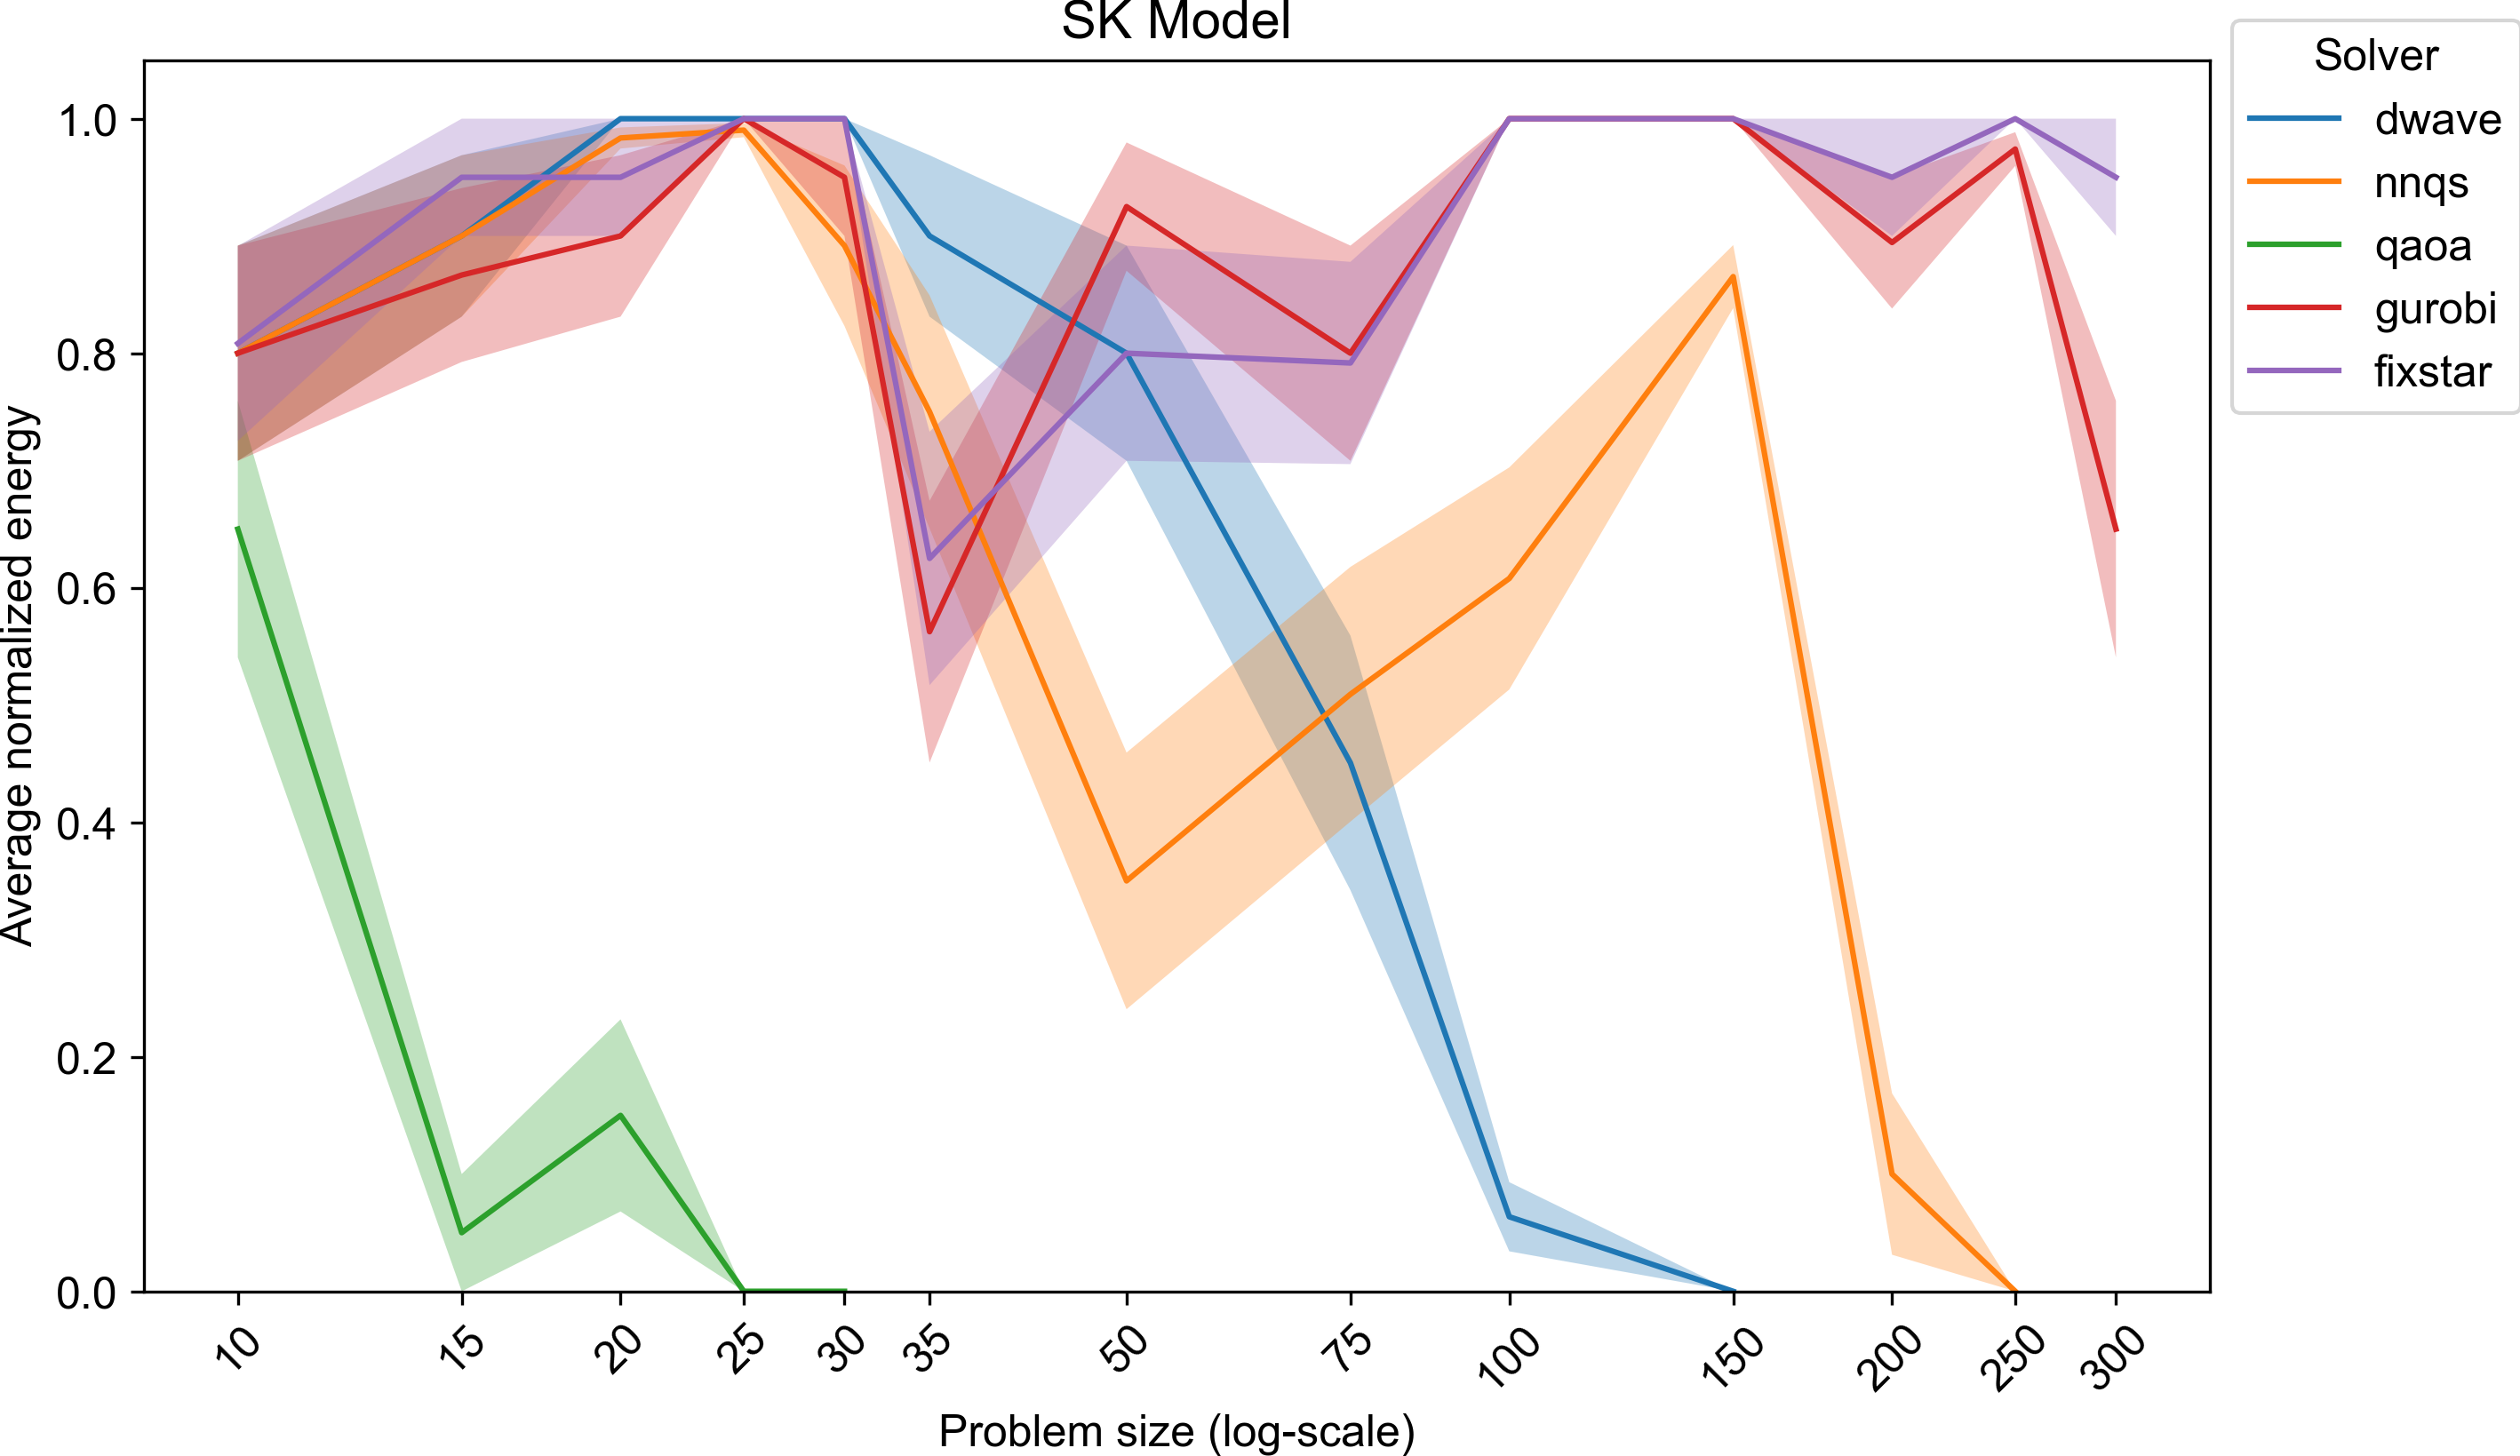
\includegraphics[width=0.9\textwidth]{images/skmodel_all_size.png}}%\hfill
    \\
    \subfloat[Success probability]{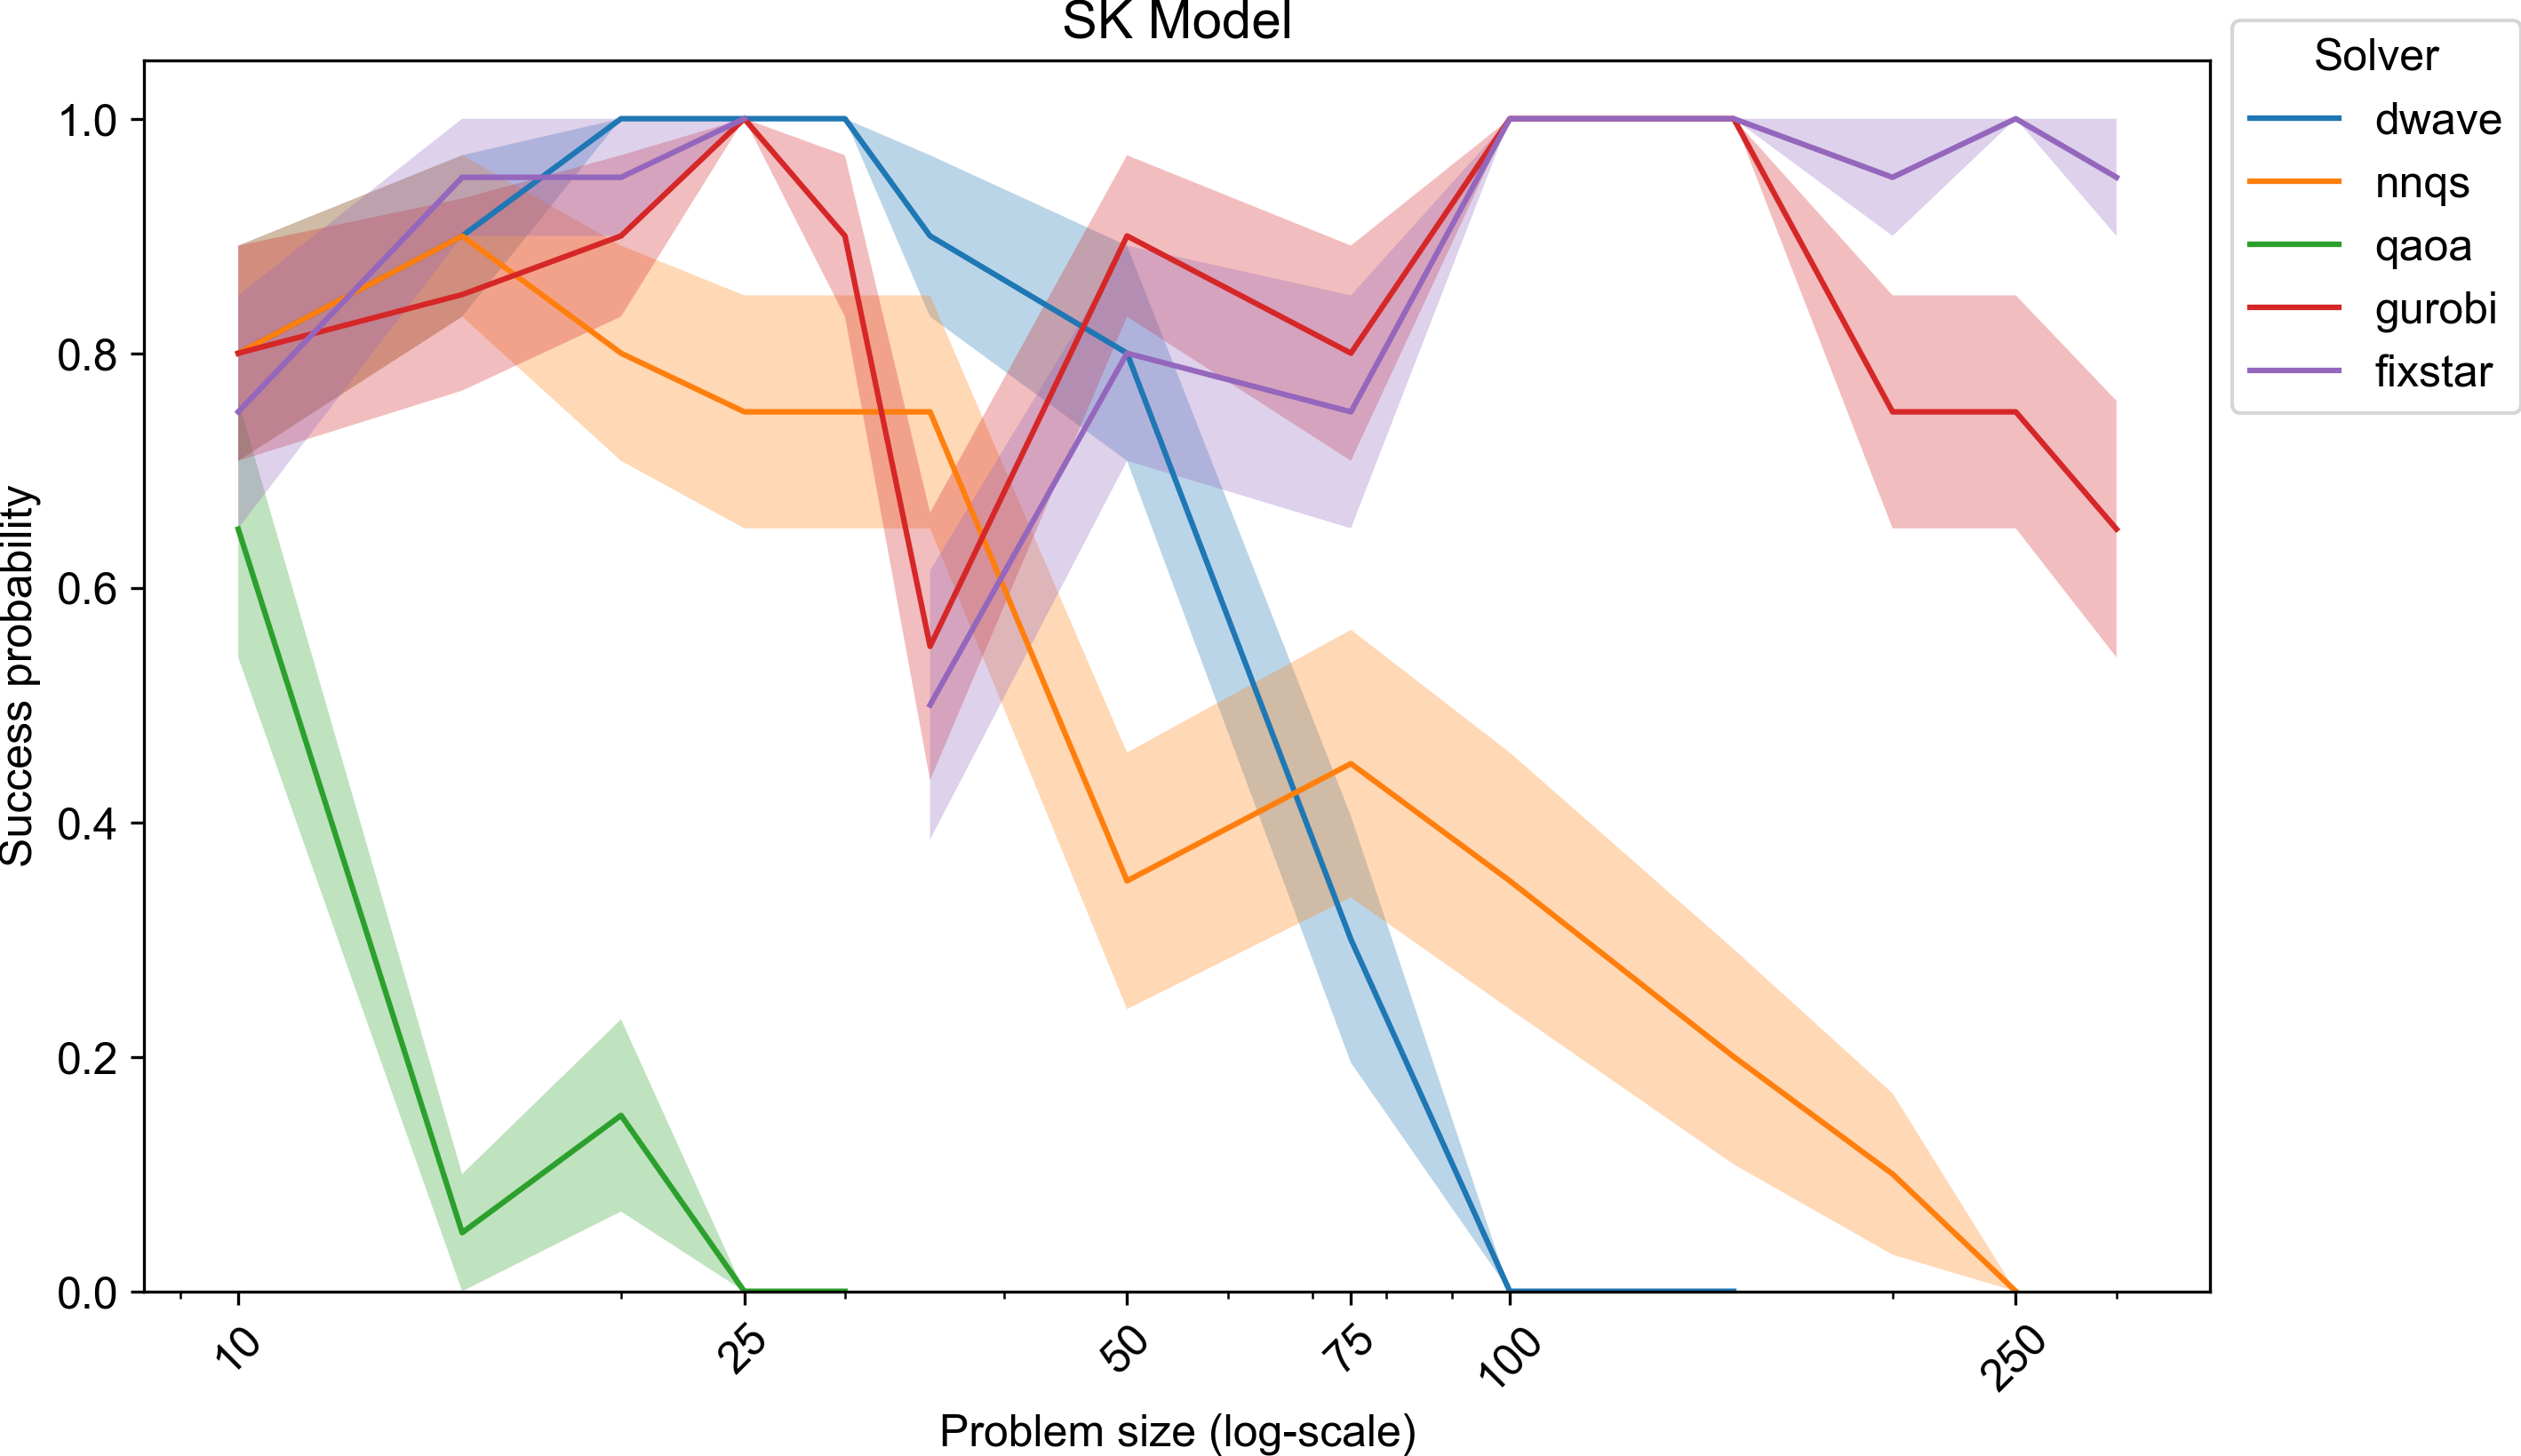
\includegraphics[width=0.9\textwidth]{images/skmodel_all_success_size.png}}
    \caption{Performance of different solvers for SK model by problem size}
    \label{all-skmodel-size}
\end{figure}

\begin{figure}[!htbp]
    \subfloat[Normalized energy]{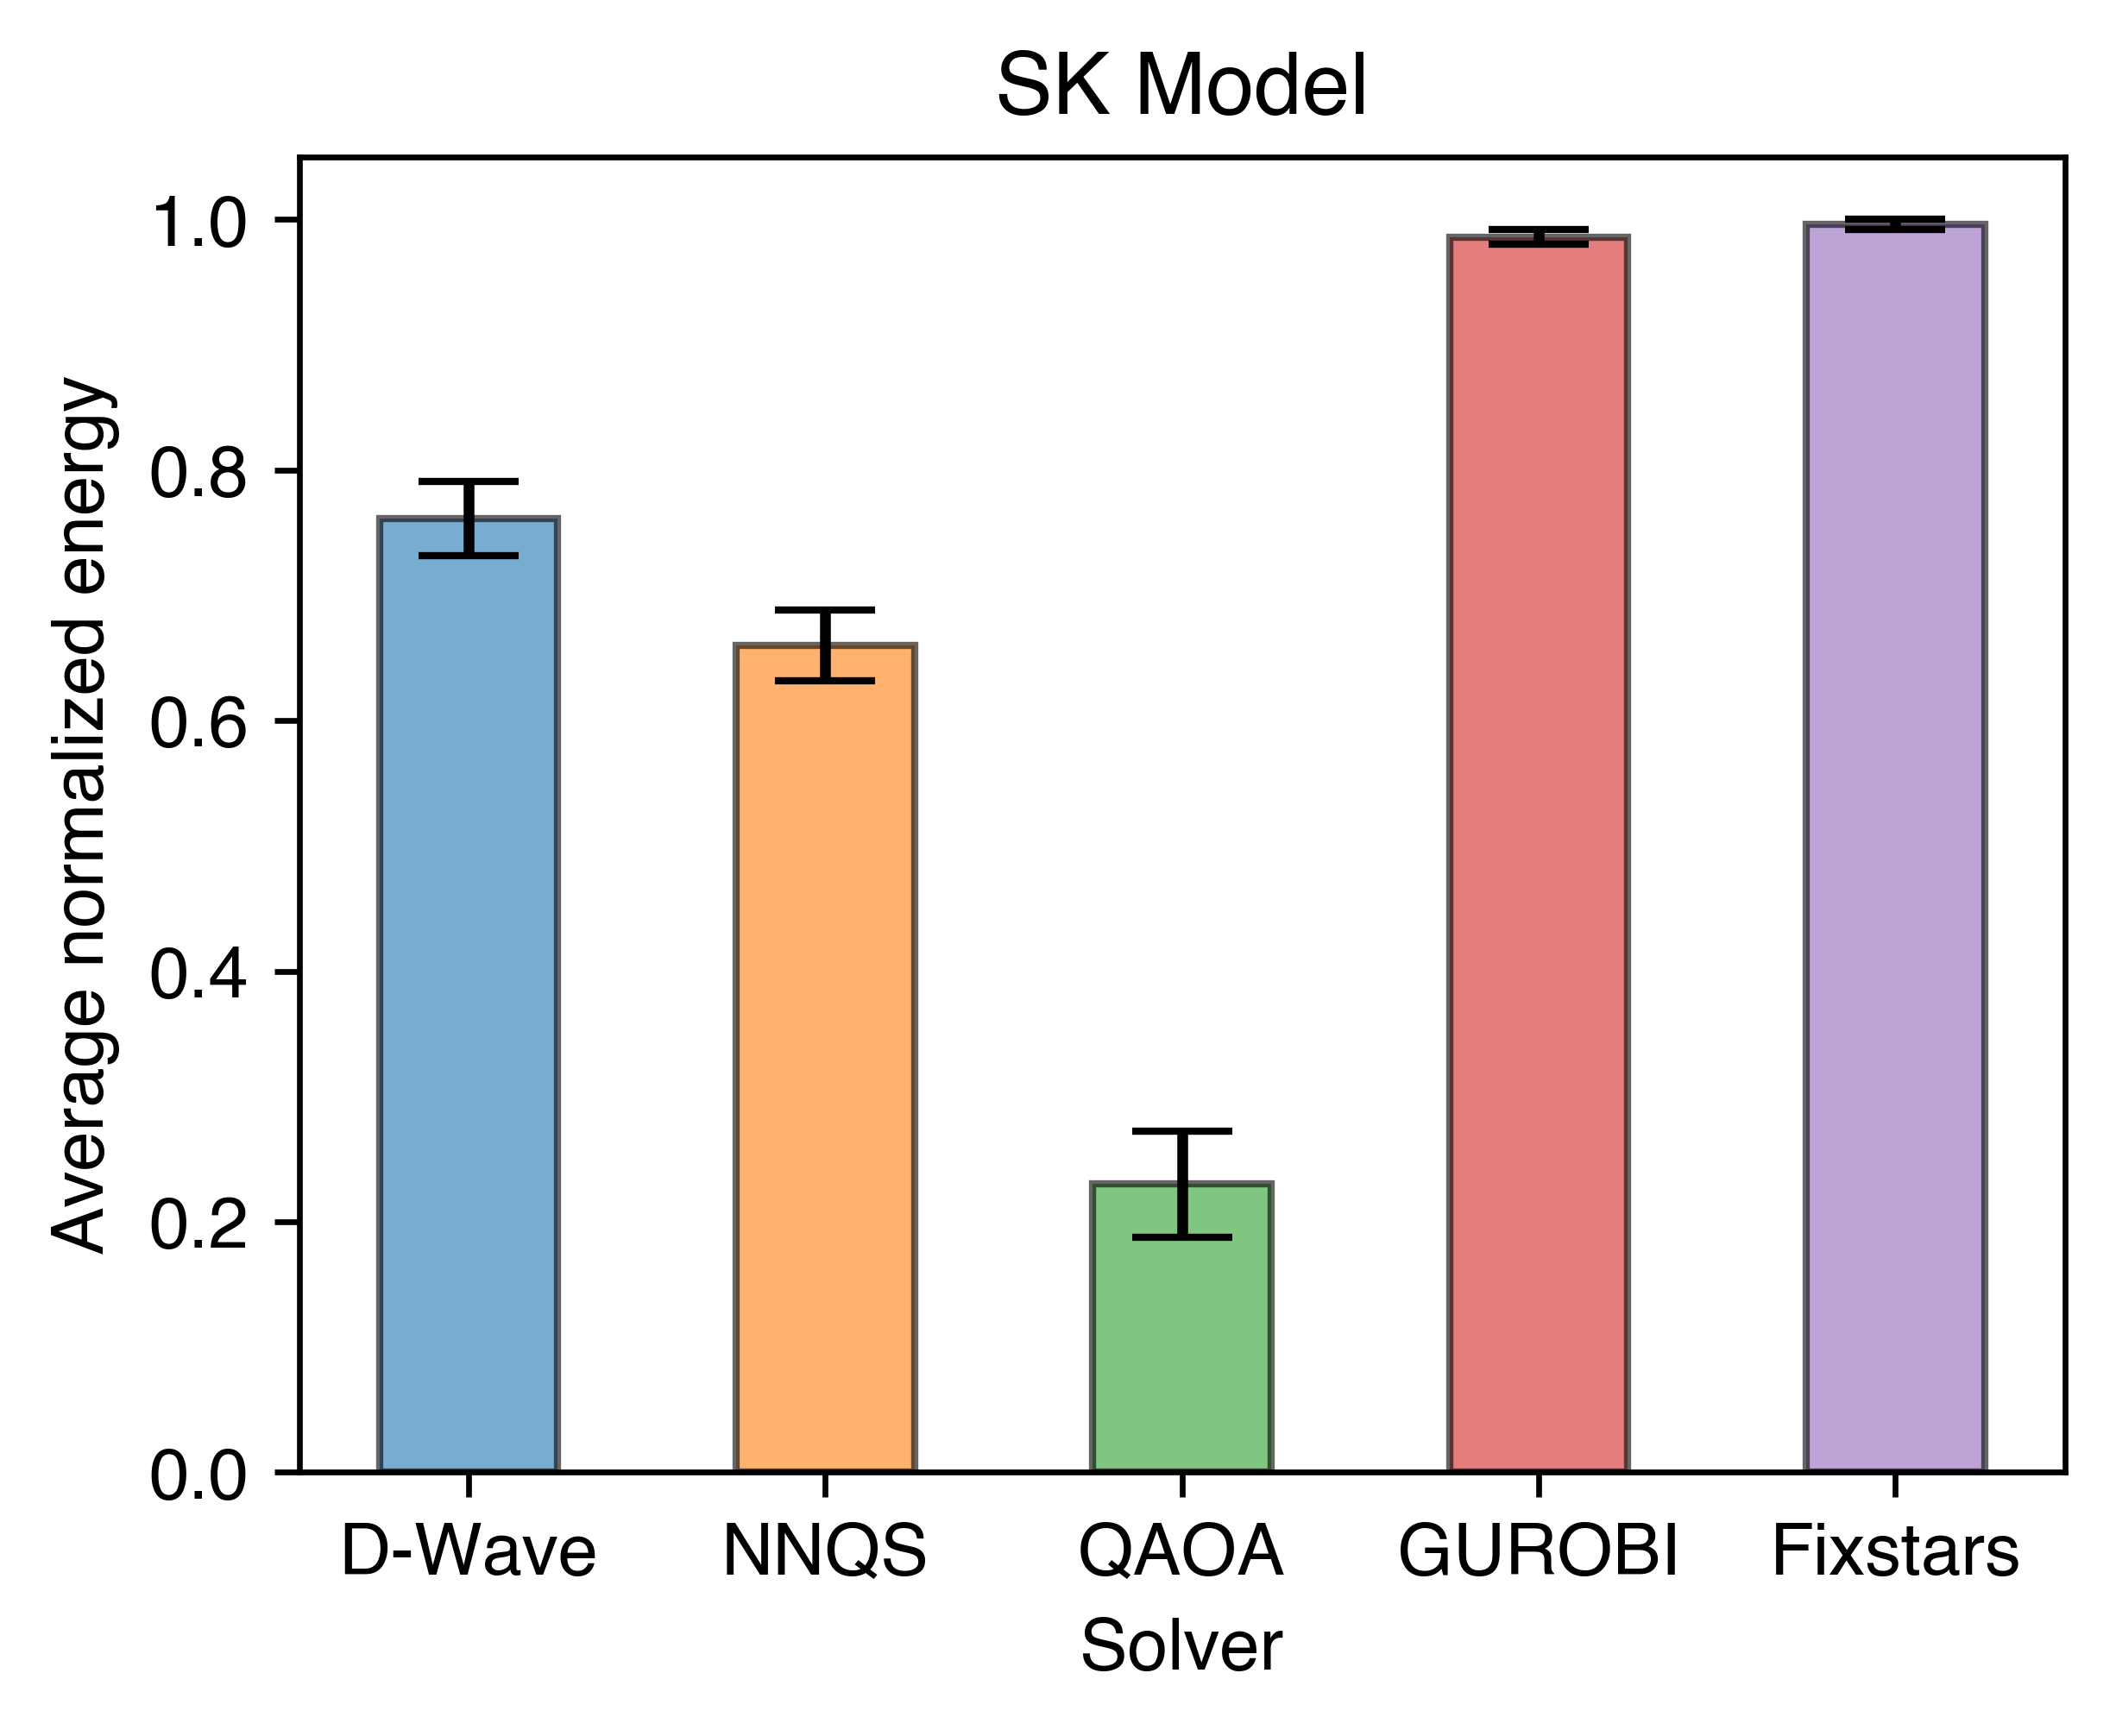
\includegraphics[width=0.49\textwidth]{images/skmodel_all_avg.png}}\hfill
    \subfloat[Success probability]{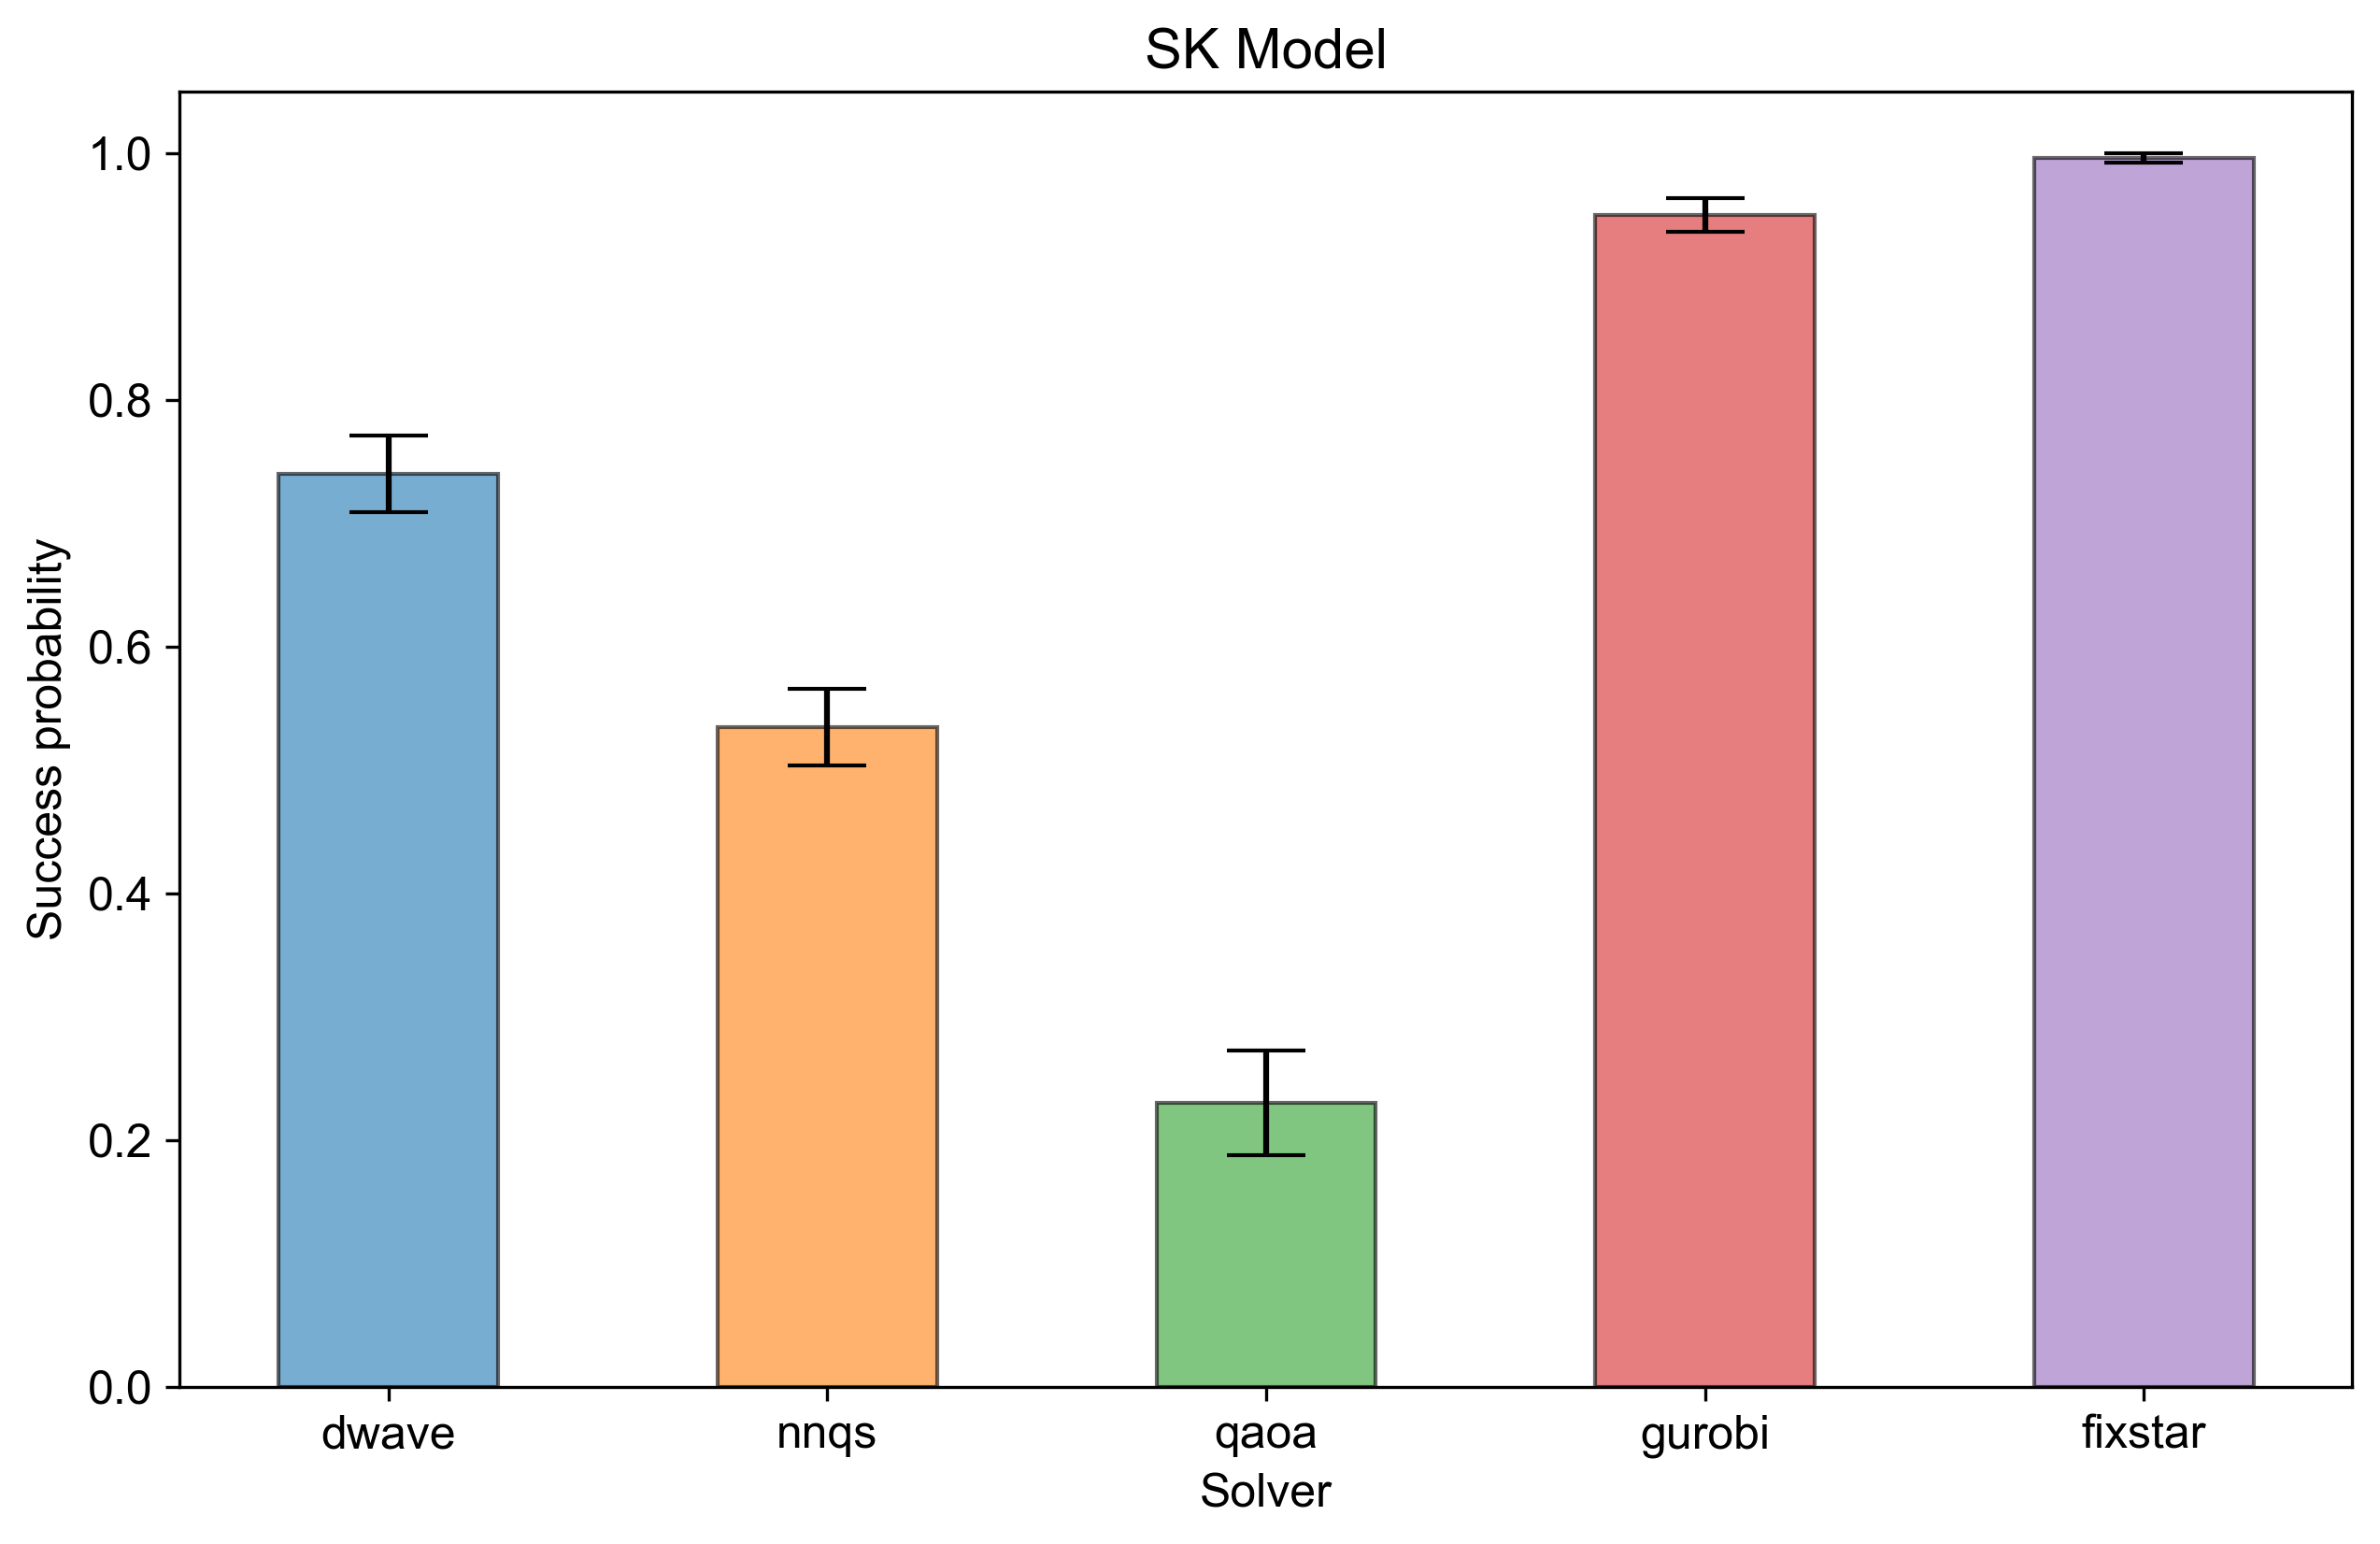
\includegraphics[width=0.49\textwidth]{images/skmodel_all_success_avg.png}}
    \caption{Average performance of different solvers for SK model}
    \label{all-skmodel-average}
\end{figure}

For the SK model dataset, the continuous training algorithm with the RBM generally performed the best in terms of normalized energy and success probability, shown in \autoref{all-skmodel-size}. The performance averaged across all sizes, shown in \autoref{all-skmodel-average}, also highlights that the RBM with a continuous training algorithm performs the best. However, it is interesting that the direct training schemes have poor performance with small problem sizes ($\leq 50$) but are relatively better at higher problem sizes ($100, 250$).

Across all the problem sets, we see that the RBM has a better average performance compared to the MLP in both average normalized energy and success probability for each training algorithm. In terms of training schemes, direct training performs the worst among the 3, and continuous training performs better than progressive training. Using the RBM with a continuous training scheme gives the highest normalized performance across all datasets.

\section{Future Work}
Future studies can explore more QUBO problem types and attempt to classify problems that are difficult for annealing-based solvers such as QA and SA but easier for other solvers such as QAOA.